\documentclass[a4paper,man, natbib,floatsintext]{apa6} %apa6/jou/man/doc
\usepackage[english]{babel}
\usepackage{csquotes}
\MakeOuterQuote{"} %will substitute " with quotes `` ''
\usepackage[utf8x]{inputenc}
\usepackage{amsmath,amssymb}
\usepackage{graphicx}
\usepackage[]{changes}
\usepackage{multicol}
\usepackage{multirow}
\usepackage{booktabs}
\usepackage{tabularx}
\usepackage{setspace}% http://ctan.org/pkg/setspace
\usepackage{url}
%This makes urls break at the end of a line
\makeatletter
\g@addto@macro{\UrlBreaks}{\UrlOrds}
\makeatother
\usepackage{rotating}
\usepackage[toc,page]{appendix}
\addto{\captionsenglish}{\renewcommand*{\appendixname}{Supplement}}
\usepackage{color}
\usepackage{subscript}
\usepackage{threeparttable}
\usepackage{threeparttablex}
\usepackage{longtable}
\usepackage{dcolumn}
\usepackage{longtable}
\usepackage{times}
\usepackage{lipsum}
% \AtBeginEnvironment{tabular}{\singlespacing}% Single spacing in tabular environment
% \AtBeginEnvironment{caption}{\doublespacing}% Single spacing in tabular environment

\graphicspath{
{../analyses/figures/}
{../experiment/materials/}
{../misc/images/}}












\title{Deconstructing financial risk perception: Perceiving risk as losses can explain a perceived negative risk--return correlation among investment options}
\shorttitle{Deconstructing financial risks}

\threeauthors{Jana B. Jarecki}{Janine Hoffart}{Jörg Rieskamp}
\affiliation{University of Basel}

% \leftheader{Deconstructing risk}


\abstract{
% % Generelle Kommenatare:
% 1. Theoretische Basis: a) Auch in der Finanzliteratur wird nicht nur Variance als Risikomass verwendet, das sollten wir klarstellen b) 2. Generell ist in der Literatur bekannt, dass Menschen Risiko unterschiedlich definieren und das es unterschiedliche Konzepte gibt. c) wir sollten das beachten und dennoch unser argument machen, dass aufgrund der unterschiedlichen Interpretationen von Risiko es wichtig wäre, bei Einschätzungen von "Risiko" spezifischer zu sein. 

% 2. Wir argumentieren ja, dass Menschen "Risk" häufig als "loss" verstehen. Wäre es dann nicht naheliegend gewesen im Experiment das Risiko auch mit einer Frage nach "losses" zu erfassen. Denn dann müsste ja ebenso eine negative Korrelation resultieren?

% 3. Begrifflichkeiten. Wir sollten einmal die zentralen Begriffe definieren und dann immer die gleiche Verwendung. Für beide Experimente würde ich sagen, dass wir immer das Risiko einschätzen lassen, dafür aber unterschiedliche Begriffe verwenden: risk-as-risk, risk-as-variance, risk-as-fluctuations etc. 



In a complex financial world, holding incorrect beliefs about the risks of investments can be disadvantageous. People commonly believe that high-risk investments bring low returns, while in many financial markets, investments with higher returns are associated with higher risks, measured as outcome variance. In two studies we examined the cognitive underpinnings of these biased high-risk--low-return perceptions. Study 1 (\textit{N} = 96) tested the high-risk--low-return perceptions as a by-product of the semantics of risk. We hypothesized and found that people understood the term "risk" to mean loss, not variance, influencing their risk perceptions. The results from quantitative statistical analysis and qualitative content analysis show that a semantic meaning of the term risk explains the high-risk--low-return perception. In Study~1, participants received information about the return on investments. Study~2 (\textit{N} = 242) removed this return information. \added{The results show that given information about the return on investment, the semantic interpretation of risk caused the biased high-risk--low-return perception, replicating Study 1. However, given no information about returns on investments, participants' high-risk--low-return perception was unaffected by semantics. Rather, without return information, negative attitudes toward investments led to the high-risk--low-return perception, which is in line with the affect heuristic.  Our results show the interaction of information about investment risks with the semantics of the term risk.} They also suggest the use of unambiguous terms (such as fluctuation) to measure outcome variance perceptions in the financial domain.}

\keywords{risk--return paradox; risk perception; attitudes; affect heuristic, risk--return belief, stock market, financial investments}

\authornote{This research is supported by a grant (SNF \# 143854) of the Swiss National Science Foundation to the second and third authors.


Correspondence concerning this article should be addressed to Jana B. Jarecki, Department of Economic Psychology, Missionsstrasse 62a, 4055 Basel, Switzerland.  E-mail: jana.jarecki@unibas.ch, jj@janajarecki.com
}

\begin{document}
\urlstyle{same}
\maketitle
%
%
Poor financial literacy is an important issue that has been making headlines for more than 80 years \citep{carrns2019,nyt1939}. Many societies strive for an economy in which everybody makes "informed financial decisions" \citep[][p. 6]{FinancialLitear2011} and much effort worldwide has been made to increase financial literacy \citep{OECD2019}. One highly important aspect of well-informed financial choices concerns people's understanding of the relationship between the benefits and risks of financial investments. Risk comprehension is considered paramount to good economic choices. To facilitate the understanding of the risks of investments, major financial institutions have started to provide potential investors with supposedly easy to understand information about the risks of investments, such as dividing risk into categories from "low risk" to "high risk" \citep[e.g., ][]{postfinance2019}, in the hope of improving people's understanding of the risks (i.e., the \textit{variance} of returns) associated with different investments.

Defining risk as the variance of returns, or semivariance of the distribution of returns on investments, is a standard approach in economic theory and finance  \added{\cite[for other common definitions of risk, see][]{Holton2004}. Risk is sometimes also understood as expected loss \citep[e.g.,][]{Kritzman2002}, but} the definition of risk as variance is widely followed by psychologists and neuroscientists \citep[e.g.,][]{Nosic2010, Coombs1960, Mishra2016,Rushworth2008, Preuschoff2006, Fujimoto2016}. \added{In particular, a common approach in the psychological literature on risky choice is to define risk as the variance of gambles}.  Any communication of "risk" in the sense of this economic notion of risk as variance requires that people also should understand financial risks in terms of variance of returns.

\subsection{A paradox in risk and return perception} Despite the efforts toward increased financial literacy, there are persistent misunderstanding of the outcome s (risk) and returns and their relation to each other \citep{Shefrin1995,Ganzach2000,Kempf2014}. Regarding the relation of outcome variances and returns, the financial market often offers a risk premium, with high-variance (risky) investments offering higher returns compared low-risk investments. Higher returns come with the costs of higher variance or risk, or in other words, the willingness to accept higher risk comes with the benefit of  higher returns, leading to a positive association between risk and returns. The positive risk--return (i.e., variance--return) relation is in line with the mean-variance model of \citeauthor[][]{Markowitz1952} (\citeyear[][]{Markowitz1952}), and it holds by and large in international stock markets \citep[][]{Dimson2003}.\footnote{In some markets there is a debate about the premium \citep[see, e.g.,][]{Figenbaum1986}.} Yet many people seem to believe not in a risk premium but in a risk punishment, judging high-risk investments as low-return investments \citep[][]{Shefrin1995, Shefrin2000, Shefrin2001, Kempf2014, Ganzach2000}. Perceiving the risk--return relationship as negative rather than positive is sometimes referred to as the  \textit{risk--return paradox} \citep[][]{Figenbaum1986}, and it has emerged as a pervasive phenomenon \citep{Kempf2014,Ganzach2000}. People's risk--return ratings have been negatively correlated in a variety of life domains besides finance, including technology and medicine \citep[e.g.,][]{Fischhoff1978, Alhakami1994,Sokolowska2015,Fleming2012}. In financial contexts, research findings have shown that even investors and economics students, who are assumed to have professional or academic expertise with risks, exhibit the risk--return paradox and rate subjectively high-risk stocks as being low-return stocks \citep{Kempf2014}. In one study \citep{Shefrin1995}, financial analysts and executives rated the returns of 10 stock market companies; they judged the companies with low variances (risk) as those with high returns. %But the calculations were per asset class rather than across assets. In the study it is not clear how risk was operationalized. In study 3 risk was operationalized as costs. Unsurprisingly a negative correlation was found for laypeople, not for experts. For stem cell treatment, the authors found a negative cost-benefit correlation for laypeople and experts.
The risk--return paradox is thus a seemingly stable cognitive bias in the perception of risks and returns in many areas of life.

In behavioral economics and decision science, one explanation for the risk--return paradox is the cognitive processing of information other than the outcome variance of options. Some research has tested if people process representativeness \citep{Shefrin1995, Shefrin2001, Pachur2012b}. The most common explanation is that people process their own attitudes toward options when forming risk and return judgments \citep[e.g.,][]{Finucane2000}. In this context, attitudes refer to a global evaluative attitude toward an investment or technology, including cognitive evaluations \citep[a global "good and bad"; ][]{Ganzach2000, Sjoerberg2007,Sokolowska2015}. In previous experiments, attitudes have been found to moderate the strength of the psychological risk--return paradox \citep{Ganzach2000, Kempf2014, Finucane2000, Slovic2004}. The core assumption of the attitude-driven explanation is that those investments that receive a generally positive cognitive evaluation should be perceived as lower in risk and higher in return, compared to more negatively evaluated investments for which a high risk and low return is predicted. This effect of general attitudes on the perception of risk and return became known as the \textit{affect heuristic} \citep{Finucane2000,Slovic2004}. It implies that people's general affective attitude toward assets should lead to a holistic evaluation of the asset and its risk and returns. Specifically, positive attitudes should lead to high-return--low-risk perceptions, and negative attitudes should lead to high-risk--low-return perceptions \citep{Ganzach2000, Finucane2000}, which as a consequence leads to a positive correlation between people's risk and return perceptions.

\added{Here, we examine an additional aspect of the processing of risks, namely semantics.} The results from semantic studies about the meaning and usage of the term "risk" have established a reliable notion of \textit{risks as losses}. In everyday language, risk often means unwanted events and their causes \citep[American English corpus from 1992 to 2012,][]{Boholm2016}. Loss, danger, and loss probabilities surround the term risk in practice. In contrast to the standard definition of risk as outcome variance in the finance literature, psychologically, risk is often understood not as variance but as a potential loss \citep[e.g.,][]{Libby1977, Sachse2012}. Even managers view risks as related to loss \citep{Mohr2010, Duxbury2004, Shapira1995}, with low positive correlations between the perceived risk and the objective variance of options' returns \citep{Weber2005,Klos2005a}. This shows that psychologically, the understanding of risk is much broader than a narrow definition of risk as variance. Therefore, we investigated if the reasonable understanding of risk as loss (the loss semantics of risk) can provide an alternative explanation of the risk--return paradox.

The semantic view of risk perception could potentially explain the risk--return paradox (the negative subjective risk--return correlation). \added{For the sake of this argument, we assume that return judgments can be made reasonably accurately because return is a less ambiguous term than risk. According to the semantic view of risk ("risk as loss"), people might interpret risk as (a) a small magnitude of the expected return, or (b) as the probability of negative returns. First consider the case in which people understand risk as low expected return \textit{magnitude}. Their resulting risk judgments should correlate negatively with their return judgments across investments, because low expected returns and high expected returns correlate negatively, by definition. In the second scenario, in which people understand risk as the \textit{probability} of losses, they may also arrive at a negative risk--return correlation. This because investments with a high probability of losses have lower expected returns than investments with a smaller probability of losses (if the variances of the returns on investments do not differ extremely). The subjective risk judgments that result from interpreting risk as loss probability should correlate negatively with their return judgments.} Therefore, the semantic view of risk can explain people's supposedly biased risk--return perception, which can be considered a correct response to their interpretation of the term risk as loss or loss probability (rather than as variance). Further, the semantic view on risk holds that people's literal "risk" judgments should reflect the real loss magnitude or loss probability, rather than the variance of returns.

We tested if the semantics of the term risk influence risk judgments, and particularly if the loss semantics of risks could explain the risk--return paradox. To this end, our experimental design elicits the perceived outcome variances (commonly elicited by "risk" judgments) of investments using different terms with different semantic connotations. Our work advances the literature on the risk--return paradox as follows: We have tested a new hypothesis about the role of semantics in the risk--return paradox; also our work is ecologically valid, because we have used real stock and fund data as material \citep[as have][]{Kempf2014}.  Additionally, because methodologically analyzing the risk--return paradox is complicated by multiple variable intercorrelations,\footnote{The correlations in the true data are such that usually, real risk correlates with real return, perceived risk correlates with real risk,  perceived return correlates with real return, perceived risk correlates with real return, and perceived return correlates with real risk; these multiple intercorrelations can be taken into account by partial correlation networks, which are the resulting pairwise partial correlations given the magnitude of the remaining correlations.} we have used partial correlation network analyses, which are specifically designed to analyze data with intercorrelations among multiple variables.


\section{Study 1}
Study~1 investigated if the loss semantics of the term risk causes the risk--return paradox in financial risk perception. Aiming to disentangle the notion of risk as loss from the notion of risk as variance, we designed the present study to manipulate the terms that people evaluated stocks by. All terms, that participants evaluated, relate to the variance of returns of investments: participants were asked about the perceived "risk" of stocks (the baseline measure), and they were asked about the "fluctuation," "variability (variance)," and "predictability" of those stocks. Predictability judgments have been shown to relate to financial risk perception \citep{Sachse2012}; the other terms represent an intuitive notion of variance, which we hoped would be associated less with loss than the term risk. Our study also assessed the perceptions of the losses and returns of stocks.


\subsubsection{Hypothesis}
We hypothesized ($H_1$) that judgments of risk would be less accurate measurements of the objective outcome variances of risky options than judgment of other terms related to outcome variance. We also hypothesized ($H_2$) that the risk--return paradox (the negative correlation between perceived risk and perceived return) is based on the semantic confusion of risk with loss and therefore that the paradox should occur mainly when people judge perceived "risk" and not when judging perceived "fluctuation," (or one of the alternative terms) that are less semantically related to loss. No hypotheses were made about which of the alternative terms (predictability, fluctuation, or variability) would lead to the most precise perception of the objective variances of risky options.

\section{Methods}
\subsection{Participants}
In total, 103 adult participants recruited from ClickWorker completed an online study. Seven were excluded (for reporting inattentiveness or the task being unclear, or using only one response option throughout a scale), leaving a final sample of $N$ = 96: 56 males and 40 females (58\% and 42\%, respectively), mean age 37 years (\textit{Mdn} = 34, $SD$ = 12, range 18--65 years). The dominant native language was German for $n =$ 90 and other for $n=6$ (94\% and 6\%, respectively). Mean study completion time was 42 min (range $10$--$120$ min), and remuneration was 4.50 euros (4.83 U.S. dollars at the time of the study). Data were collected in May 2017. The study was approved by the institutional review board at the University of Basel. All participants possessed a secondary school degree, and $n$ = 37 had a bachelor’s or higher degree. Most participants worked full or part time, and $n=10$ were students.

\subsection{Task Design}
The study used a $1 \times 4$ (Question Wording [risk, fluctuation, predictability, variability (variance)]) within-subject design. Participant rated 19 stocks that were presented graphically one by one (see Materials). Participants rated the perceived risk, perceived predictability, perceived fluctuation, and perceived variability (variance) of all stocks. Participants also evaluated the stocks' expected loss, loss magnitude, loss probability, and return. Table \ref{table:Questions} shows the questions.

% Wie hoch schätzen Sie das Risiko der gezeigten Aktie ein? Wie hoch schätzen Sie die Variabilität (Varianz) der gezeigten Aktie ein? Wie hoch schätzen Sie die durchschnittliche Schwankung der Rendite der gezeigten Aktie ein? Wie hoch schätzen Sie die Vorhersagbarkeit der Rendite der gezeigte Aktie ein (gemessen ab 2003)?

\begin{table}[hb!]
\centering
\onehalfspacing
\begin{threeparttable}
\caption{Conditions (within-subject) and question wording in Study 1}
\small
\label{table:Questions}
\begin{tabularx}{\columnwidth}{p{1.7cm}p{2.9cm}p{7cm}r{0.5cm}}
Category & Condition & Question & Response format \\
\toprule
\multirow{7}{*}{Variance} & Risk & How high do you estimate the risk of the displayed stock to be? & 7--point Likert \\
& Variability & How high do you estimate the variability (variance) of the displayed stock to be? & 7--point Likert \\
&  Fluctuation & How high do you estimate the average fluctuation of the displayed stock returns to be? & 7--point Likert \\ 
 & Predictability & How high do you estimate the predictability of the displayed stock (starting from 2003) to be? & 7--point Likert \\
 \cmidrule{2-4}
\multirow{7}{*}{Loss} & Expected loss & How high do you estimate the expected average loss of this stock to be? &  $\%$ points \\
     & Loss magnitude & How high do you estimate the average loss of this stock to be? & $\%$ points\\
     & Loss probability & How high do you estimate the probability of taking a loss with this stock in a randomly selected year to be?\\
 \cmidrule{2-4}
\multirow{1}{*}{Return} & Return magnitude & How high do you estimate the average return of this stock to be? & 7--point Likert \\
\bottomrule
\\
\end{tabularx}
\begin{tablenotes}
\small
\item
 \textit{Note}. The original question wording was in German (see Supplement~\ref{sup:study1_material}). Likert-type scales were unipolar from \textit{1 = extremely low} through \textit{4 = moderate} to \textit{7 = extremely high}, except the return scale, which was bipolar from \textit{1 = extremely large losses} to \textit{7 = extremely large gains}.

\end{tablenotes}
\end{threeparttable}
\end{table}

\subsection{Procedure} The experiment was a computerized online study. Participants were familiarized with 19 stocks, each of which presented graphically (Figure~\ref{fig:study1_material}). The stock graphs were unlabeled to avoid familiarity effects. Participants evaluated each stock individually (e.g., evaluating "risk") on a Likert-type scale (from \textit{1 = low} through \textit{4 = moderate} to \textit{7 = high}). After the evaluation of all stocks, participants evaluated the stocks with respect to a different term (e.g., "risk" in Block 1, "fluctuation" in Block 2, etc.). The orders of the terms and stocks were randomized across participants. Participants were instructed to make relative judgments among the set of stocks to avoid use of external reference anchors. Participants also evaluated the stocks' return and loss (numerical inputs from 0 to 100). Further, the participants defined risk (\textit{What does it mean to you if a stock has "high risk?"}), reported their stock market experience and knowledge, took a graph literacy test \citep{Garcia-Retamero2013a}, and reported demographics. Data-quality checks followed (comprehension of instructions, self-reported quality). Participants had to pass an attention-check question before each block to ensure they knew what to evaluate next. Participants saw only the return history of the stocks but no names of the stocks, to avoid familiarity biasing risk--return judgments \citep{Ganzach2000}.

\subsection{Stimuli}
The stimulus material was based on real stock market data to ensure ecological validity. Study~1 used the daily point values of the 19 most-traded stocks in Switzerland (as of October 2016, between January 2003 and December 2015, see Supplement~\ref{sup:study1_material}). To characterize the stocks, we computed the stocks' objective annual nominal returns, variance in returns, and their losses. Our  measure of return was the stock's change in value after a 1-year holding period (ignoring inflation), for each day of a calendar year, averaged within calendar years.\footnote{The return on investment (ROI) of each stock was calculated as the percentage earnings between end and start values when selling after 1 year, for example, for 2006: $ROI_{\text{2006}} = \frac{v_{2007}^{\text{close}} - v_{\text{2006}}^{\text{open}}}{v_{\text{2006}}^{\text{open}}}$, where $v_y$ is the stock value in year $y$ at the start and end of the trading day ($v^{\text{open}}$, $v^{\text{close}}$, respectively), correcting for bank holidays. If it was a bank holiday the next trading day was used. The returns within a calendar year were averaged, yielding one percentage return for each year.}
Information about the stimuli (in terms of the computed annual nominal returns on investment) was provided to participants for evaluation in the form of a graphic (year by return, as a percentage; Figure~\ref{fig:study1_material}). Participants were informed about the meaning of the return that the graphic displayed in the instructions (see Supplement~\ref{sup:study1_material}).

\begin{figure}[h!] \centering
    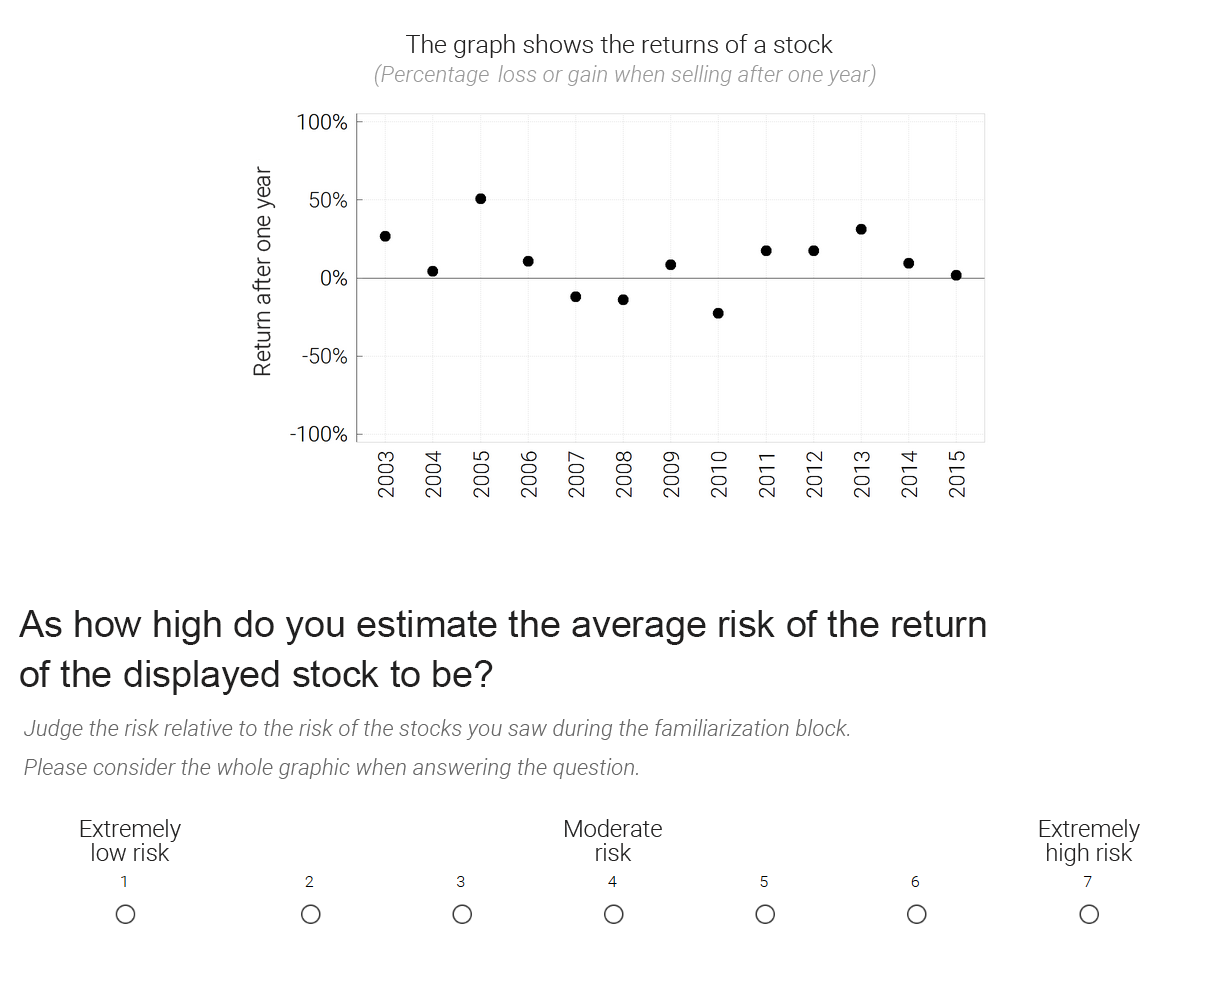
\includegraphics[width=0.85\textwidth]{fig1}
    \caption{\textit{Illustration of the task in Studies~1 and 2.} The original language of the study was German  (original wording: Supplement~\ref{sup:study1_material}). The English translation was added for this publication only. During Study~1, each participant evaluated 19 stocks with respect to the variance-related terms in Table~\ref{table:Questions}: variability, risk, fluctuation, and predictability.}
    \label{fig:study1_material}
\end{figure}

\subsection{Analytic Approach}
% wäre es nicht gut zunächst mit deskriptiven ergebnisse anzufangen bevor Du hier das mixed-effects model erklärst und die effekte testest?
% JJ > solved this 
We examined which of the terms (risk, fluctuation, variability, predictability) characterizing the risk of an investment led to the most accurate judgments of the stocks' risk defined by the variance of the stocks' returns. Before presenting the results (next section), we describe the analytic approach. To analyze the condition-related differences in the accuracy of people's judgments of the true outcome variance (\textit{H}\textsubscript{1}), we used a linear model comparison among models that predicted the true outcome variance from the judgments in the conditions \citep[following][]{Judd2017}.\footnote{The regressions included the predictors Question Condition $+$ Evaluation $+$ Condition $\times$ Evaluation interaction, and a by-participant random intercept and random slope to account for the clustering in the data, because the design of Study~1 has fully crossed explanatory variables (each participant evaluated each stock in each condition once).}
%
To analyze the effect of the question wording on the risk--return paradox (\textit{H}\textsubscript{2}), we used linear models to estimate the effect of the perceived risk (fluctuation, variability, and predictability) on the perceived return \citep[following][]{Judd2017,Barr2013a}.\footnote{We included as many random effects as model convergence allowed \citep[following][]{Judd2017,Barr2013a} The regressions predicted the perceived return from: Perceived Variance (\textit{z} standardized) $+$ Condition (effect coded) $+$ Perceived Variance $\times$ Condition $+$ Stock Return $+$ Stock Return $\times$ Condition, including random effects (by-participant intercept $+$ by-participant slope for Perceived Variance $\times$ Condition; uncorrelated random intercept and slope). The condition was effect coded: Effect coding means that the coefficients represent the deviation from the grand mean rather than from a reference level. Technically, effect coding involves coding categorical variables such that the coefficients sum to zero, which facilitates the interpretation of interactions \citep[e.g.,][]{Singmann2019}.} %
%
In a second, more fine-grained, analysis we modeled partial correlations among the variables using partial correlation networks \citep[e.g.,][]{Epskamp2019}, which estimate the conditional dependencies between multiple variables while controlling for the dependencies among the remaining variables. This second analysis accounts for the interdependencies among the variables perceived risk, objective risk, perceived return, and objective return, in ways other than regressions.\footnote{We used a network model that account for the clustering in our within-subject design). We employed a random-intercept model. The latest hierarchical network model, \citep[v0.4.3;][]{Epskamp2019}, only allows random intercepts.} Also, we ran robustness checks, using subgroup analysis (see below). Last, to gauge the relationship between participants' explicit definitions of risk and the strength of their risk--return paradox, we combined qualitative content analysis wtih linear modeling of the risk--return paradox.

All analyses were conducted in R \citep[v3.6.1;][]{R}, using the packages lme4 \citep[v1.1;][]{Bates2015} and mlVAR \citep[v0.4.3;][]{Epskamp2019}. Likert-type scale responses were \textit{z} standardized by participant to control for differences in scale use, except where stated otherwise, for a lack of convergence of models.

\subsection{Results}
\subsubsection{Accuracy of the terms related to outcome variance}
How well do the four terms by which participants evaluated the stocks (risk, fluctuation, variability [variance], and  predictability) represent the order of magnitude of the objective outcome variances of the stocks? \textit{H}\textsubscript{1} expects the perceptions of risk to be the least accurate measure of the objective variances compared to the perceptions of predictability, fluctuation, or variability. The size of the Pearson correlations between the stocks' objective outcome variance and people's perceptions follow this rank order: fluctuation $>$ variability $>$ predictability $>$ risk ($r_{fluct}=.69$, $r_{vari}=.64$, $r_{pred}= -.52$, $r_{risk}= .49$, respectively), pooled across participants and stocks (statistical tests can be found in Supplement~\ref{study1_risk-variance-correlation}). The mixed-effects regression model comparison (Table \ref{tab:study1_lm_results}) reveals that, as hypothesized, the model that includes perceived risk as a predictor of the objective outcome variances has the worst fit, and the best fitting model uses perceived fluctuation as a predictor of objective variance, as indicated by log likelihood, Akaike information criterion (AIC), and Bayesian information criterion (BIC), evidence strength \citep[the best model has an AIC weight of 1; see][]{Wagenmakers2004}. The regression coefficients show that all perceived values were positively related to the objective variance of the returns of the shown stocks. The highest standardized $\beta$ coefficient was obtained for perceived fluctuation ($\beta = 0.64$, 1 \textit{SD} change in the objective variance given 1 \textit{SD} change in the predictor, not shown in Table 2); the $\beta$s of variability, predictability, and risk were lower, $ 0.57, -0.39$, and $0.29$, respectively. These results support \textit{H}\textsubscript{1}, according to which when asking people for the risk of an investment their evaluation is not necessarily highly correlated with the variance of the asset's returns. Thus, questions about the risk of an asset do not lead people to evaluate the variance of the assets' returns, which is also in line with \citeauthor{Klos2005a}'s (\citeyear{Klos2005a}) results.


% Table created by stargazer v.5.2.2 by Marek Hlavac, Harvard University. E-mail: hlavac at fas.harvard.edu
% Date and time: Fr., Mai 17, 2019 - 10:13:52
\begin{table}[!htbp] \centering 
  \caption{Hierarchical linear model results, dependent variable: objective variance of shown stocks} 
  \label{tab:study1_lm_results} 
\begin{tabular}{@{\extracolsep{5pt}}lcccc} 
\\[-1.8ex]\hline 
\hline \\[-1.8ex] 
 & \multicolumn{4}{c}{Unstandardized b coefficients [range of dep. var. 0.014 $-$ 0.275]} \\ 
\cline{2-5} 
\\[-1.8ex] & (1) & (2) & (3) & (4)\\ 
\hline \\[-1.8ex] 
 Fluctuation & .028 &  &  &  \\ 
  & (.027, .030) &  &  &  \\ 
  & t = 32.413$^{***}$ &  &  &  \\ 
  & & & & \\ 
 Variability &  & .026 &  &  \\ 
  &  & (.024, .028) &  &  \\ 
  &  & t = 28.657$^{***}$ &  &  \\ 
  & & & & \\ 
 Predictability &  &  & $-$.017 &  \\ 
  &  &  & ($-$.019, $-$.015) &  \\ 
  &  &  & t = $-$17.359$^{***}$ &  \\ 
  & & & & \\ 
 Risk &  &  &  & .021 \\ 
  &  &  &  & (.018, .023) \\ 
  &  &  &  & t = 15.006$^{***}$ \\ 
  & & & & \\ 
 Constant & $-$.040 & $-$.026 & .158 & .009 \\ 
  & ($-$.048, $-$.031) & ($-$.034, $-$.017) & (.150, .165) & ($-$.003, .021) \\ 
  & t = $-$9.148$^{***}$ & t = $-$6.068$^{***}$ & t = 40.864$^{***}$ & t = 1.522 \\ 
  & & & & \\ 
\hline \\[-1.8ex] 
AIC weight$^{+}$ & 1.00 & 0.00 & 0.00 & 0.00 \\ 
AIC & -5458 & -5373 & -5027 & -4887 \\ 
BIC & -5425 & -5340 & -4994 & -4854 \\ 
LogLik & 2735 & 2692 & 2519 & 2449 \\ 
\hline 
\hline \\[-1.8ex] 
\textit{Note:}  & \multicolumn{4}{l}{$^{*}$p$<$0.05; $^{**}$p$<$0.01; $^{***}$p$<$0.001} \\ 
 & \multicolumn{4}{l}{$^{+}$Relative evidence strength, range 0-1 {\citep{Wagenmakers2004}}} \\ 
 & \multicolumn{4}{l}{Predictors are z-transformed} \\ 
 & \multicolumn{4}{l}{Model: random intercept and slope by subject; fit: restricted maximum likelihood.} \\ 
\end{tabular} 
\end{table} 

%% JR had a comment here, that got lost - ask him.

\subsubsection{The loss semantics of risk and the risk--return paradox}
In line with past work on the risk--return perceptions, we expected to observe a negative correlation between the perceptions of the returns and risks of the stocks in the risk condition (where participants evaluate "risk.") In contrast, in the other three conditions in which alternative terms were used to elicit the judgment of the stocks' variances in returns, we expected a positive correlation between perceived return and perceived alternative measure of risk. Objectively, the nominal returns of the stocks used in Study~1 showed a risk premium, as theoretically expected; that is, stocks with a larger return had a higher risk, mesured as variance in return: objective $r_{\text{risk,return}} = .51$, 95\% confidence interval (CI) $[0.07$, $0.78]$, $p = .027$, pooled across stocks (Figure~\ref{fig:rrc}a). Figure~\ref{fig:rrc}b shows the perceived returns in relation to the perceived risk, variance, fluctuation, and predictability. As hypothesized and unlike the objectively positive risk--return correlation, perceived "risk" correlated negatively with perceived return ($r = -.14$), exhibiting the risk--return paradox. However, perceived fluctuation and perceived variability correlated positively with perceived return ($r = .10$, $r = .11$, respectively) and thus are more in line with the objective correlation. Perceived predictability was only weakly correlated with perceived return ($r = -.03$). Inferential statistics of the simple correlations are given in Supplement~\ref{study1_supplementary_results}, Table~\ref{sup:tab:study1_rrc}. In sum, although the correlations between the perceived return and perceived variability/fluctuation ($.10$ and $.11$) are smaller than the objective correlation ($.51$), they are in the right direction, showing people's general understanding of the true variance--return relationship when they are asked in a more precise way, rather than asked about "risk". 
%
\begin{figure}[!htbp] 
 \centering
 \fitfigure[]{fig2.png} 
  \caption{\textit{Objective risk--return relationship compared to perceived "risk"--return relationship across different terms related to variance}. (a) Objective risk--return relation: Returns increase with variances across the stocks. (b) Perceived relations between the perceived returns of stocks and perceptions of four terms related to variance ("perceived values"): perceived \textit{risk}, perceived \textit{variability}, perceived \textit{fluctuation}, and perceived \textit{predictability} (measured on 7-point Likert-type scales, \textit{z} standardized at the individual level). Lines depict best fitting linear regressions, pooled across participants.}
  \label{fig:rrc}
\end{figure}

The results of our regression analysis\footnote{For the regression model, see the section on analytical approach. The maximal mixed-effects model, which some recommend using \citep{Barr2013a}, has a more complex random effects structure \citep[see][]{Judd2017}. Specifying this full model caused singularity, i.e., degenerate parameter estimates, which is a convergence issue common to mixed-effects models involving by-participant \textit{and} by-stimulus random effects \citep{Bates2015b}. Singularity issues can severely distort the interpretation of the parameters \citep{Bates2015b}. Thus, we simplified our model by following recommendations for mixed-effects modeling when the interaction is of interest \citep{Barr2013a}. Moreover, the full model also includes correlated random intercepts and slopes. A model with those also failed to converge, but simulations showed low Type I error rates for uncorrelated random effects \citep{Matuschek2017}.}
reveal that, as hypothesized, only in the "risk" condition do the perceived returns decrease with the perceived risks ($b_{\text{risk}}=-0.159$). In the fluctuation or variability condition, $b_{\text{fluct}}=0.086$ and $b_{\text{vari}}=0.086$, the correlations with perceived returns were positive (all $p$s$<.05$, Table~\ref{study1:mixed_effects_model}). The perceptions of predictability were not significantly related to the perceptions of return. Similarly, the results from the partial correlation network analysis show the risk--return paradox exclusively for perceived "risk," and for none of the other terms. Perceived risk decreased with perceived return ($r_{part} = -.15$, $p < .001$; Figure~\ref{fig:pcn}a). \added{Network analyses go beyond regressions in also analyzing which variables predict the independent variables in addition to the dependent variable \citep{Epskamp2018a}; the network results estimate the six partial correlations that are possible with four variables (objective return and risk, and perceive return and risk).} The results from the network analysis corroborate the results from the linear regression analyses.

% In Table 3 werden auch signifikante positive Effekte für Fluctuation und Variability aufgezeigt, diese sollten wir dann auch hier nennen.

% JJ: Alle Effekte aus Table 3 werden im Text beschrieben. Ich denke Du meinetest Figure 3 (?)

\begin{table}[H]
\begin{center}
\begin{threeparttable}
\caption{Regression (mixed-effects model) with dependent variable: perceived return \\\label{study1:mixed_effects_model}}
    \begin{tabular}{lrcrcrr}
    \toprule
    Term & $b$ & 95\% CI & $b^*$ & \textit{df} & \textit{t} & \textit{p}\\
    \midrule
    Constant & 4.604 & [4.456, 4.763] & --$-$ & 95.005 & 60.936 & $<$ .001\\
    Perception & 0.009 & [-0.032, 0.051] & 0.007 & 375.787 & 0.455 & .650\\
    Perception $\times$ Risk & -0.159 & [-0.226, -0.097]  & -0.084 & 178.275 & -4.716 & $<$ .001\\
    Perception $\times$ Fluctuation & 0.086 & [0.013, 0.156] & 0.046 & 164.840 & 2.445 & .016\\
    Perception $\times$ Variability & 0.086 & [0.015, 0.153] & 0.046 & 150.384 & 2.325 & .021\\
    \bottomrule
    \addlinespace
    \end{tabular}
\begin{tablenotes}[para]
\normalsize{\textit{Note.} \textit{b} $=$ unstandardized fixed effect; \textit{b}$^*$ $=$ standardized fixed effect; \textit{df} $=$ degrees of freedom (Satterthwaite); confidence intervals (CIs) are bootstrapped (500 runs); condition main effects are excluded, because the criterion was measured once for all within-subject conditions and thus did not vary across conditions.}
\end{tablenotes}
\end{threeparttable}
\end{center}
\end{table}

\begin{figure}[H] 
 \centering
 \fitfigure[]{fig3.png} 
  \caption{\textit{Partial correlation networks.} Shown are partial correlations between perceptions of return and perceptions of risk, fluctuation, variation, and variability---controlling for the correlations between the other variables. \textit{Line width} $=$ association strength; \textit{dashed line} $=$ negative association; \textit{missing line} $=$ nonsignificant association  $\geq \alpha=.05/4=0.0125$ to correct for the four variables. Shown are within-subject paths, i.e., how each participant's deviations from the means predict each other for the same stock \citep[contemporaneous effects; ][]{Epskamp2018}.}
  \label{fig:pcn}
\end{figure}

\subsection{Perceived Risk as Amount and Probability of Loss}
\added{
To explore the relationship between risk perception and loss in more detail, we analyzed loss-related variables \citep[e.g., probability and amount of loss, ][]{Kritzman2002}. Table \ref{tab:cor_risk_loss} lists the simple correlations between participants' perceptions of "risk" and three aspects of loss: the mean amount of loss across years [$\sum$L$/$n($L$), where $L$ is a loss amount and n($L$)  is the count of years with losses]; the probability of a loss [n($L$)$/$n(years)]; and the expected loss [P(loss)$\times$Mean(loss)],  which were computed from the objective returns shown to participants. Table \ref{tab:cor_risk_loss} shows that the perceived risk correlates more highly with the mean loss ($r=.54$) and the expected loss ($r=.57$) than with the probability of loss ($r = .17$). This suggests that the magnitude of losses might be related to the perception of risks more than the probability of losses.
}

\begin{table}[tbp]
\begin{center}                     
\begin{threeparttable}                         
\caption{Simple correlation of perceived risk with objective return and loss}
\label{tab:cor_risk_loss}

                                                                                     
\begin{tabular}{lllllll}
\toprule                                                                             
 & & \multicolumn{3}{c}{Objective}  &\\                                                
\cmidrule(r){3-5}                                                                    
 & \multicolumn{1}{c}{1} & \multicolumn{1}{c}{2} & \multicolumn{1}{c}{3} & \multicolumn{1}{c}{4} & \multicolumn{1}{c}{$M$} & \multicolumn{1}{c}{$SD$}\\                   
\midrule                                                                             
(1) Perceived risk & - &  &  &  & 0.00 & 1.38\\                                      
(2) Return & .10*** & - &  &  & 0.10 & 0.07\\                                        
(3) Mean(loss) & .54*** & .00 & - &  & 0.19 & 0.09\\                                 
(4) \textit{P}(loss) & .17*** & -.44*** & .03 & - & 0.37 & 0.08\\                             
(5) \textit{EV}(loss) & .57*** & -.19*** & .93*** & .38*** & 0.07 & 0.04\\             
\bottomrule                                                                          
\addlinespace                                                                        
\end{tabular}                                                                        
                                                                                     
\begin{tablenotes}[para]                                                             
\normalsize{\textit{Note.} * $p <$  .05; ** $p < $ .01; *** $p < $ .001. Perceived risk values are mean-centered by individual. \textit{EV}$=$ expected value}                                                                          
\end{tablenotes}                                                                     
                                                                                     
\end{threeparttable}                                                                 
\end{center}                                                                         
                                                                                     
\end{table}

\subsubsection{Qualitative content analysis: the semantics of risk}
Our last analysis examines individuals' explicit notions of risk using the qualitative data. The open-ended responses to \textit{"what does high risk mean to you?"} were categorized following qualitative content analysis principles \citep{Mayring2014} with an interrater reliability of $\kappa = .85$.\footnote{A research assistant deductively created a coding manual, which was refined inductively after categorizing 25 sample responses; the research assistant and J.H. coded the remaining statements independently} The qualitative analysis resulted in a loss category that included statements such as "High risk means that you lose money with high probability"\footnote{Original German statement: "Hohes Risiko bedeutet, dass man mit hoher Wahrscheinlichkeit Geld verlieren kann."}; a variance-related category had statements such as "High risk, to me, means high volatility" and "The return varies a lot"\footnote{Original German: "Hohes Risiko bedeutet für mich hohe Volatilität" and "Die Rendite schwankt stark."}; the "other" category contained statements such as "I would not buy it" and "One cannot simply say this."\footnote{Original German: "Würde nicht kaufen" and "Kann man so nich sagen."}

The frequency of categories shows that $n=65$ (47.2\%) responses related risk to notions of losses; only $n=
19$ (13\%) of the responses defined risk as variance and another group of $n=20$ (12.5\%) related risk to uncertainty (Table~\ref{table:QualRisk1}). These results are in line with previous work on risk perception \citep[e.g.,][]{Mohr2010, Duxbury2004}. Moreover, the subset of participants who defined risk as related to loss were more prone to the risk--return paradox (risk--return correlation $r=-.19$) compared to those who did not mention losses in the open-ended question ($r=-.01$): simple correlations of risk and return perceptions given the mention of loss $r_{\text{"loss"}} = -.19$, 95\% CI $[-.24$, $-.13]$, $t(1214) = -6.59$, $p < .001$; and $r_{\text{Not "loss"}} = -.01$, 95\% CI $[-.08$, $.07]$, $t(606) = -0.14$, $p = .892$. These results corroborate the results from our correlation network analyses, that the representation of the term risk as "losses" facilitates the risk--return paradox.

\begin{table}
\centering
\begin{threeparttable}
\caption{Categorized open-ended responses to "What does risk mean to you?"}
\small
\label{table:QualRisk1}
\begin{tabular}[12cm]{lrrlrr}
% latex table generated in R 3.6.0 by xtable 1.8-4 package
% Fri Jun 14 11:58:40 2019
Category & \textit{N}$^a$ of 141 & Relative$^b$ & Group & Group \textit{N}$^a$ & Group relative$^b$ \\ 
  \midrule
Uncertainty &  20 & 12.5\% & Uncertainty &  20 & 12.5\% \\ 
  Variance, fluctuation &  19 & 13.0\% & Variance, fluctuation &  19 & 13.0\% \\ 
  Loss: Probability &  17 & 13.4\% & Loss &  65 & 47.2\% \\ 
  Loss: Magnitude &  16 & 10.2\% &  &  &  \\ 
  Loss: Probability + Magnitude &  17 & 13.4\% &  &  &  \\ 
  Loss: Other &  15 & 10.2\% &  &  &  \\ 
  Gain: Probability &   5 & 4.0\% & Gain &  26 & 15.8\% \\ 
  Gain: Magnitude &  14 & 8.0\% &  &  &  \\ 
  Gain: Probability + Magnitude &   5 & 3.0\% &  &  &  \\ 
  Gain: other &   2 & 0.9\% &  &  &  \\ 
  Danger &   1 & 1.0\% & Danger &   1 & 1.0\% \\ 
  Other &  10 & 10.4\% & Other &  10 & 10.4\% \\ 
   \bottomrule
\end{tabular}

\begin{tablenotes}
\renewcommand{\TPTminimum}{\linewidth}
\def\tnote#1{\protect\TPToverlap{\TPTtagStyle{#1}}}%
\small
\textit{Note.}\\
    \item[$^a$] The sum equals 141 because statements of 33 (6) participants fell into two (three) categories.\\
    \item[$^b$] Multiple-category correction was applied, weighting those falling into two (three) categories by $\frac{1}{2}$ ($\frac{1}{3}$).

\end{tablenotes}
\end{threeparttable}
\end{table}

\subsubsection{Robustness checks}
 The ability to read graphs (graph literacy) and stock market experience were added to the analyses as robustness checks for the results. Domain knowledge can safeguard against the risk--return paradox \citep[e.g.,][]{Fleming2012}. Participants' self-reported general stock market experience and experience with the Swiss stock market, which were measured on a 5-point Likert-type scale, were averaged into an experience score for each participant. The median participant had an experience score of 1.5 ($M=1.76$, $SD=0.81$, range 1--4). The data were split at an experience level of 2 into a relatively inexperienced group ($n=55$) and a medium to highly experienced group; the partial correlation network analysis was repeated for the subgroups, with results that confirm our main results (only risk perception shows the risk--return paradox, correlation of risk and return perceptions for the inexperienced: $r_{part}=-.15, p < .001$; experienced $r_{part}=-.10, p < .001$; see  Supplementary Figure~\ref{fig:study1_pcor_by_exp}). Regarding graph literacy, it may be that participants correctly interpreted risk as variance but could not read graphs correctly. Their median graph literacy score was 10 (10 correct answers out of 13, indicating good graph literacy, $M=10.25$, $SD=3$, range 3--13). We split the data at the median graph literacy score into high- and low-literacy groups. The correlations between risk and return judgments were reanalyzed with partial correlation networks, as outlined above. Individuals with low graph literacy ($n=54$) still show the risk--return paradox, with perceived risk correlating negatively with perceived returns, $r_{part} = -.14, p  <  .001$. By contrast, the highly graph literate group shows no correlation between perceived risks and perceived returns. But they still confused risk with "loss," judging the stocks that had objectively low returns as having high risk, objective-return--perceived-risk partial correlation, $r_{part}=-.17, p < .001$. All coefficients can be found in the Supplementary Figure~\ref{fig:study1_pcor_by_glit}. We did not control for the joint occurrence of experience level and graph literacy because the resulting subgroups were too small to reliably estimate the partial correlations.

In summary, these robustness checks show that perceptions of "risk" lead to a subjectively negative risk-return correlation across levels of experience, and for participants who are less able to read graphs, whereas perceptions of "fluctuation" are most robustly capturing the true positive variance--return relationship across experience and graph literacy. 

\subsection{Discussion of Study~1}
Taken together, our quantitative and qualitative results suggest that the interpretation of risk as loss (loss semantics of risk) strongly influences the risk--return paradox, that is, the negative correlation between perceived risk and return. We found the negative perceived risk--return correlation for the evaluation of stocks when asking people to evaluate the outcome variance of stocks by the term "risk." In contrast, when we asked participants to judge the variance of the stocks by the term "fluctuation," a positive correlation between perceived fluctuation and return emerged. Participants' perceptions of fluctuation and return were unbiased compared to the objective variance--return correlations, and this was because perceptions of fluctuation represented the objective outcome variances more accurately than perceived risk and because of the lack of loss semantics for the term fluctuation.

% Use "variance" judgment rather than "risk" judgement.

The data show furthermore that the order of the objective variances in stock returns is measured least accurately by perceptions of risk and most accurately by perceptions of \textit{fluctuation}. In our data, the risk perception of stocks was a mixture of the perceptions of the true outcome variances and the true losses of the stocks. We recommend that researchers who are interested in the elicitation of variance perceptions in risk research consider measuring the perceived fluctuation of the options.


\section{Study 2}
\added{The design of Study~1 informed participants about the objective nominal returns of the stocks that they evaluated, which we relaxed in Study 2.} In Study~2 we aimed to replicate Study~1 with new material and to take a closer look at three aspects of the loss semantics of risk: (a) Does a definition of risk as variance overwrite the semantic risk--loss association and thus eliminate the risk--return paradox? Previous work has used qualifications such as "risk (measured as variance)" \citep[e.g.,][]{Kempf2014a}.\footnote{The authors asked about future risk by asking "How risky (where risk should be estimated based on the return variance of the firm’s stock) do you estimate this firm to be over the next 12 months relative to all other firms of the DAX30?" \citep[][p. 1007]{Kempf2014}.} (b) What is the impact of graphical information? In Study 1, graphical information about the stocks' returns was provided and might have had a major impact on the observed results. Therefore in Study 2 we examined the impact of this information by omitting the graphical information in one experimental condition. (c) What is the role of attitudes, which have been shown to matter in previous research, when measuring fluctuation? As outlined in the Introduction, global attitudes are expected to moderate the risk--return paradox. A strong positive attitude, particularly toward unfamiliar options, should lead to perceptions of low risk and high returns as predicted by the affect heuristic \citep[][]{Finucane2000}.

\section{Methods}
The design of Study~2 resembles that of Study~1, but Study~2 employed a between-subjects design and used one new term in the variance-related questions; two terms were identical to those in Study~1 \added{the questions were formulated as in Table \ref{table:Questions}}. In one between-subjects condition the participants simply had to evaluate the "risk" of the options; in the second condition the participants judged the "fluctuation" (as in Study 1). In the new condition the participants had to evaluate the "risk (measured as variance)." Study~2 used different stocks as stimuli (see Stimuli below).

\subsection{Task Design}
Study~2 used a 3 $\times$ 2 between-subjects design (Question Wording [risk, risk (measured as variance), and fluctuation] $\times$ Graph [shown, hidden]), with the covariate attitudes. Participants were randomly assigned to one of the three conditions.

\subsection{Participants}
The sample size was determined beforehand. In total, 269 participants recruited from ClickWorker completed an online study; 27 were excluded (for inattentiveness, not following instructions, zero response variance on scales, and being underage), leaving a final sample of $N = 242$; 133 males, 107 females and 2 other (55\%, 44\% and 1\%, respectively), mean age 36 years (\textit{Mdn} $ = 34$, \textit{SD} $= 10$, range 18--61 years). The native language was mostly German ($n = 228$, 94.2\%), followed by 6 other, 3 no answer, 2 English, 2 Swiss German,  and 1 Italian (2.5\%, 1.2\%, 0.8\%, 0.8\%, and 0.4\%, respectively). The mean study completion time was 33.7 min (range $9.4$--$165$ min). Remuneration was 4.50 euros (\$4.83 at the time of the study). Data were collected during August and September 2017. The study was approved by the institutional review board at the University of Basel. Table~\ref{tab:study2_subsample} lists the characteristic of the groups by condition.

While all participants were informed about the name and country of origin of the funds, only the participants in the graph condition received information about the yearly returns (Figure~\ref{fig:study1_material}); in the no-graph condition participants saw only the name and country of the fund. 

% latex table generated in R 3.5.0 by xtable 1.8-3 package
% Mon May 27 17:53:45 2019
\begin{table}[ht]
\centering
\caption{Study~2: Descriptive statistics for each between-subjects condition}
\label{tab:study2_subsample}
\begin{tabular}{lrrrccc}
\toprule
  Condition & \textit{n} & \textit{M} Age & \textit{SD} Age & \% Female & \textit{M} Financial literacy \\ 
    \toprule
    & \multicolumn{5}{c}{Graph}\\
   \cmidrule{2-6}
   Risk &  40 & 39.08 & 9.94 & 50\% & 7.10 \\ 
   Risk (measured as variance) &  42 & 36.19 & 9.25 & 48\% & 7.81 \\ 
   Fluctuation &  40 & 36.85 & 11.06 & 48\% & 7.42 \\ 
   \midrule
  & \multicolumn{5}{c}{No graph}\\
  \cmidrule{2-6}
  Risk &  41 & 32.56 & 9.24 & 36\% & 7.54 \\ 
  Risk (measured as variance) &  39 & 35.69 & 11.06 & 24\% & 7.44 \\ 
  Fluctuation &  40 & 37.23 & 11.06 & 60\% & 7.42 \\ 
   \bottomrule
\end{tabular}
\end{table}

\subsection{Procedure}
The procedure followed Study~1: Evaluations of the stocks in terms of risk, risk-as-variance, and fluctuation were measured on Likert-type scales (Table~\ref{table:Questions}); the stimulus material were index funds. In addition to the evaluations, participants rated their attitudes toward the countries of origin of the funds; this measure was to maximize useful responses, because the names of some index funds consisted of abbreviations that would be potentially unknown to the general population. Attitudes were measured on a 5-point four-item semantic differential with endpoints \textit{good/bad}, \textit{interesting/boring}, \textit{strong/weak}, and \textit{active/passive} \citep{Kempf2014}.

\subsection{Stimuli}
The stimuli were 20 international index funds traded in the 20 most-traded global currencies during the years 2007 to 2016 (as of 27 June 2017, listed in the Supplement Table~\ref{tab:study2_material}). The name and country of the funds were shown as, for example, \textit{Index from the USA (Dow Jones Industrial Average Index)}. As in Study~1, the objective annual returns on investment were computed for each index fund, providing us with an objective measure of the returns, losses, and outcome variances of the stimuli.

\subsection{Analytical Approach}
The main analytical approach followed that in Study~1. In the network analyses we added attitudes as a new predictor. To examine the mediating effect of the strength of positive attitudes on the strength of the risk--return paradox, we followed the mediation method of \citeauthor{Imai2010} (\citeyear{Imai2010}) in mixed-effects model with affect as mediator variable and the predictors estimations, graph, wording condition, the condition-graph-estimation interaction and by-subject random intercepts \citep[using the R package mediation, v4.4.7;][]{tingeley2014}.

\subsection{Data Processing}
The five-item attitude scale was transformed into an attitude score for each participant and country \citep{Kempf2014a}\footnote{The labels \textit{good, interesting, strong}, and \textit{active} were taken as positive scale endpoints.}; the mean Cronbach's $\alpha$ was $.81$ across indices/countries ($Mdn =.81$, $SD=.03$, range .77--.89). Attitude scores were centered for the mediation analysis; the evaluations of risk, risk-as-variance, and fluctuation were \textit{z} standardized at the individual level, unless otherwise stated.

\subsection{Results}
\subsubsection{Accuracy}
One purpose of Study 2 was to test if an explicit definition of risk as variance improves the accuracy of the judgments of objective outcome variance. In the graph condition, the objective variances were correlated with perceived risk-as-variance ($r_{\text{{riskasvar}} = .53$), risk ($r_{\text{risk}} =.46$), and fluctuation ($r_{fluct} = .75$), pooled across participants and stimuli. Without graphs, the correlations were lower, yet positive for perceived fluctuation ($r=.36$), risk ($r=.30$), and risk-as-variance ($r=.25$; for pooled simple correlations and inferential tests, see Supplement~\ref{study2_subj_obj_cor}). Table~\ref{tab:study2_hlm_trends} shows the results of regressing the objective variance on perceptions; post hoc trend analyses showed a significantly higher main effect of evaluations with graphs (trend $=0.077, p < .001$) compared to without graphs (trend $=0.040, p < .001$); $\Delta_{\text{graph-no.graph}}=0.037$, $p<.001$. Fluctuation had a larger  (marginal) effect than risk (trend $\Delta=.039$, $p<.001$), and than risk-as-variance ($\Delta=.029$, $p < .001$), but the effects of risk and risk-as-variance were not reliably different from each other ($\Delta=.096$, $p=.236$). Without graphs, the marginal effects of evaluations on objective risks were indistinguishable from each other (see Table~\ref{tab:study2_hlm_trends_pairwise}). These results show that \added{explicitly qualifying the term risk as variance (by asking about "risk (measured as variance)") did not improve the accuracy of participants' judgments in terms of the correlation with the objective variances of the funds.}


% latex table generated in R 3.6.0 by xtable 1.8-4 package
% Mon Jun 17 13:07:24 2019
\begin{table}[ht!]
\centering
\caption{Hierarchical linear model results---trend analysis with dependent variable: objective risk (variance of the index funds)} 
\label{tab:study2_hlm_trends}
\begin{tabular}{lcccc}
  \toprule
Question & Trend & $SE$ & $z$ ratio & $p$ \\ 
  \midrule
& \multicolumn{4}{c}{Graph}\\
\cmidrule{2-5}
  Risk & 0.061 & 0.004 & 14.278 & $$<$$.001 \\ 
  Risk (measured as variance) & 0.070 & 0.004 & 16.952 & $$<$$.001 \\
   Fluctuation & 0.100 & 0.004 & 23.438 & $$<$$.001 \\ 
   \midrule
& \multicolumn{4}{c}{No graph}\\
\cmidrule{2-5} 
  Risk & 0.039 & 0.004  & 9.337 & $$<$$.001 \\ 
    Risk (measured as variance) & 0.033 & 0.004  & 7.723 & $$<$$.001 \\ 
  Fluctuation & 0.047 & 0.004  & 11.112 & $$<$$.001 \\ 
   \bottomrule
\multicolumn{5}{l}{\rule{0em}{2.5ex}{\footnotesize \textit{Note. }Degrees-of-freedom method: asymptotic}.}\\
\end{tabular}
\end{table}
%

\subsubsection{The risk--return paradox}
Does qualifying the term risk diminish the risk--return paradox? For the index funds used in Study~2, the funds' objective risk (defined as variance of returns) and the funds' returns correlated positively with each other, $r = .63$, 95\% CI $[.26$, $.84]$, $t(18) = 3.44$, $p = .003$; see Figure~\ref{fig:study2_rrc}a. In contrast, in the condition with graphs, the perceived returns were negatively related to the perceived risks  ($r_{risk} = -.19$) and also negatively related to the perceived risk-as-variance ($r_{\text{riskvar}}=-.10$); that is, we replicated the risk--return paradox. Furthermore, qualifying risk as variance did not eliminate the risk--return paradox. As in Study~1, when asking participants about the risk of the funds by asking for the "fluctuation," we observed a positive correlation between "fluctuations" and "returns" ($r_{\text{fluct}} = .19$), pooled across participants and stimuli (for inferential statistics, see Table~\ref{table:supplement_tab1}). Without graphs, however, the risk--return paradox emerged for risk ($r = -.22$) and risk-as-variance ($r= -.19$), but now also for fluctuation ($r=-.39$); see Figure~\ref{fig:study2_rrc}b (for statistical tests, see Table~\ref{tab:study2_rr}). \added{The fluctuation judgments without graphs were positively correlated with the fluctuation judgments with graphs ($r_{\text{with,without}}=.60$), but the return judgments without graphs were not significantly correlated with the return judgments with graphs ($r_{\text{with,without}}=.01$; correlation of the mean judgments by fund).} Regression results\footnote{Dependent variable: perceived return. Predictors/fixed effects: perceived outcome variance (\textit{z} standardized) $+$ wording condition (effects coded) $+$ graph condition (effects coded) $+$ Wording Condition $\times$ Graph Condition interaction $+$ Wording Condition $\times$ Graph Condition $\times$ Perceived Variance interaction. Random effects: by-subject intercept \citep[For an explanation of effects coding, see][]{Singmann2019}} revealed that only in the graph condition were perceived fluctuation and perceived return positively related, as hypothesized, but this relation was not significant (most likely because Study~2 had lower power compared to Study~1). The size of the marginal effects of fluctuation on return perception in Study~2 ($b=0.172$) was almost two times higher than the effect in Study~1 ($b=0.095$). Without graphs and contrary to the semantic view of risk, there was a negative relation of all perceived risk concepts (risk, risk-as-variance, and fluctuation) with perceived return, exhibiting the risk--return paradox consistently. These negative marginal effects on return perception did not differ in size across the wording conditions ($\Delta_{\text{riskasvar-fluct}}=0.167$, $p=.414$; $\Delta_{\text{riskasvar-risk}}=0.012$, $p=.996$; $\Delta_{fluct-risk}=-0.155$, $p=.457$). These results show that information matters in the elimination of the risk-return paradox.

%
\begin{figure}[h!] 
 \centering
 \fitfigure[]{fig4.png} 
  \caption{\textit{Study 2: Objective risk--return relationship compared to perceived "risk"--return relationship for three terms related to variance}. (a) The objective risk (variance of the funds) correlates positively with returns on investment. (b) Shown are the relation between the perceived return and the terms related to variance: risk, risk-as-variance, and fluctuation (measured on 7-point Likert-type scales, \textit{z} standardized at the individual level), split by whether graphical information about return history was provided. Lines depict best fitting linear regressions, pooled across individuals.}
  \label{fig:study2_rrc}
\end{figure}
%

\clearpage

\subsection{The Role of Attitudes}
The attitude ratings had a median across participants of $3.5$ out of maximally 5 points ($M=3.44$, $SD=0.89$, range 1--5). Norway was evaluated most positively, on average, and Turkey least positively ($M=3.95$ and $2.73$, respectively).

Figure~\ref{fig:study2_mediation_paths} and Table~\ref{tab:study2_mediation} show the results of the mediation analysis regarding the influence of attitudes on the perceived risk--return relationship. The affect heuristic \citep{Finucane2000} posits that, across assets, negative attitudes produce \added{a higher risk and a lower return perception. Attitudes should therefore mediate the effect of risk on return perception.} We found a mediation only in the risk and risk-as-variance conditions; for fluctuation, attitudes suppressed an otherwise positive fluctuation--return association (with graphs). In both "risk" conditions, positive attitudes partially mediated the perceived risk--return relationships: "Risk" had an unmediated effect of $b=-0.24, p=.009$ on return perceptions, which was weakened to $b=-0.20, p=.022$ through the mediator attitudes (with graphs). Perceived "risk (measured as variance)" had a negative but insignificant association with perceived returns originally ($b=-0.11$), but the effect size diminished significantly with the mediation ($b=−0.09$), with graphs, in line with the affect heuristic. Importantly, perceived "fluctuation" had a positive but not substantial unmediated effect on return perception ($b=0.17$), which was not mediated but boosted by adding the indirect effect through affect ($b=0.19, p=.028$), with graphs. Thus, when measuring fluctuation, stronger positive attitudes suppressed a positive perceived fluctuation--return association. Therefore, there is an interaction between attitudes and fluctuation perception, rather than a mediation of the fluctuation--return relationship through affect. This is only partially in line with the affect heuristic: \added{When we asked for "risk" and "risk (measured as variance)," the data supported a mediation of the negative risk--return relation by attitudes, supporting the affect heuristic. But when we asked for "fluctuation," the data supported a suppression of a positive risk--return relation by attitudes.}.

\begin{figure}[H]
    \centering
    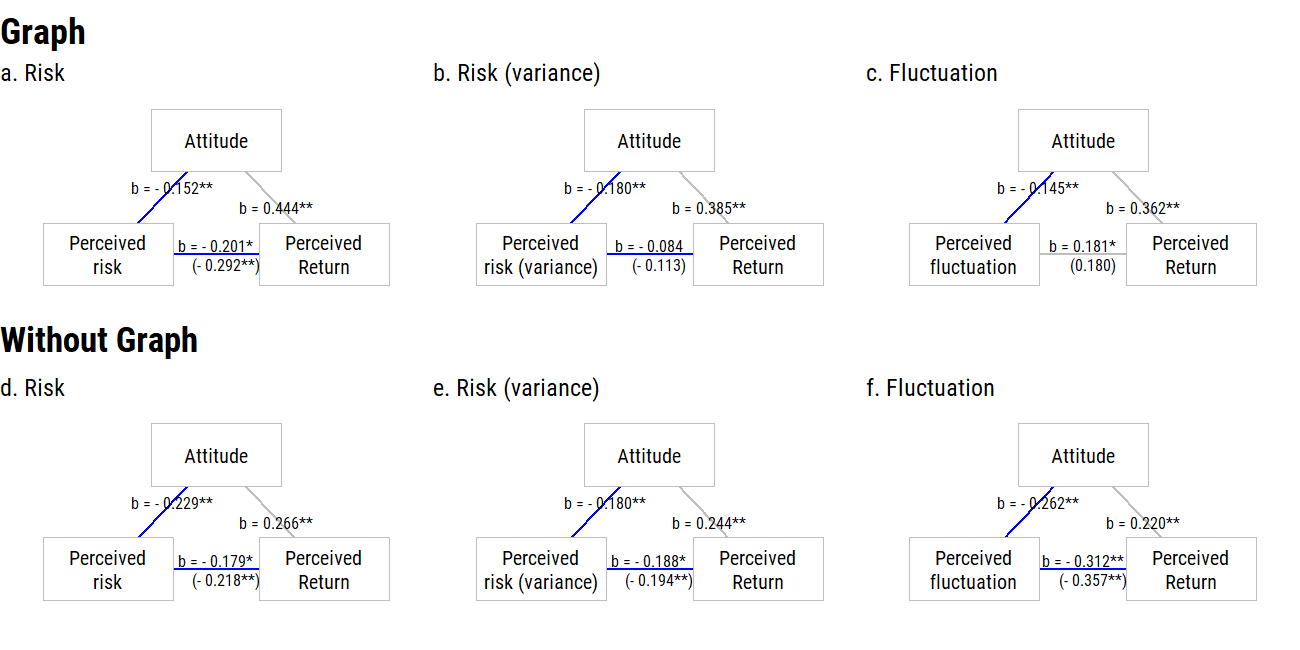
\includegraphics{fig7}
    \caption{\textit{Study 2: Attitude mediation effects by condition.} \textit{Blue lines} = Negative paths. For more details, see text and mediation effects in Table~\ref{tab:study2_mediation}.}
    \label{fig:study2_mediation_paths}
\end{figure}


\begin{table}[H]
\begin{threeparttable}
    
    \caption{\label{tab:study2_mediation}Mediation analysis with dependent variable: perceived risk; mediator: attitude score}
    \centering
    \fontsize{9}{10}\selectfont
    \begin{tabular}{@{}l@{\hspace{2mm}}r@{\hspace{2mm}}c@{\hspace{2mm}}r@{\hspace{4mm}}r@{\hspace{2mm}}c@{\hspace{2mm}}r@{\hspace{4mm}}r@{\hspace{2mm}}c@{\hspace{1mm}}r}
    \toprule
    \multicolumn{1}{c}{ } & \multicolumn{3}{c}{Mediation effect} & \multicolumn{3}{c}{Direct effect} & \multicolumn{3}{c}{Total effect} \\
    \multicolumn{1}{c}{ } & \multicolumn{3}{c}{IV $\rightarrow $ A $\rightarrow$ R} & \multicolumn{3}{c}{IV $\rightarrow$ R} & \multicolumn{3}{c}{} \\
    \cmidrule(l{3pt}r{3pt}){2-4} \cmidrule(l{3pt}r{3pt}){5-7} \cmidrule(l{3pt}r{3pt}){8-10}
      IV & \textit{b} & 95\% CI & \textit{p} & \textit{b} & 95\% CI & \textit{p} & \textit{b} & 95\% CI & $p$\\
    \midrule
    \addlinespace[0.3em]
    & \multicolumn{9}{c}{Graph}\\
    \cmidrule{2-10}
    Risk & $-$0.069 & [$-$0.11, $-$0.03] & $<$.001 & $-$0.200 & [$-$0.37, $-$0.03] & .022 & $-$0.295 & [$-$0.48, $-$0.12] & .004\\
    Risk (m. as var.) & $-$0.068 & [$-$0.10, $-$0.03] & $<$.001 & $-$0.088 & [$-$0.26, 0.08] & .326 & $-$0.167 & [$-$0.34, 0.00] & .062\\
    Fluctuation & $-$0.052 & [$-$0.09, $-$0.02] & $<$.001 & 0.187 & [0.01, 0.35] & .028 & 0.133 & [$-$0.04, 0.29] & .154\\
    \midrule
    & \multicolumn{9}{c}{No graph}\\
    \cmidrule{2-10}
    Risk & $-$0.059 & [$-$0.09, $-$0.03] & $<$.001 & $-$0.176 & [$-$0.34, $-$0.01] & .042 & $-$0.256 & [$-$0.43, $-$0.08] & .002\\
    Risk (m. as var.) & $-$0.044 & [$-$0.07, $-$0.02] & $<$.001 & $-$0.182 & [$-$0.37, $-$0.01] & .032 & $-$0.230 & [$-$0.42, $-$0.06] & .008\\
    Fluctuation & $-$0.058 & [$-$0.09, $-$0.04] & $<$.001 & $-$0.314 & [$-$0.50, $-$0.13] & $<$.001 & $-$0.401 & [$-$0.59, $-$0.21] & $<$.001\\
    \addlinespace[0.3em]
    \bottomrule
    \end{tabular}
    \begin{tablenotes}\small
        \textit{Note.} IV = Independent variable; mediation effect = indirect effect of the IV on return perception through the mediator attitudes, IV $\rightarrow$ A $\rightarrow$ R; direct effect = effect of the IV on return perception not transmitted through the mediator attitudes, IV $\rightarrow$ R. \textit{b} = unstandardized effect. CI = confidence interval; m. as var. = measured as variance. Results are based on 1,000 simulation runs per condition (6,000 runs).
    \end{tablenotes}
\end{threeparttable}
\end{table}

\subsection{Discussion of Study 2}
In summary, the results from Study~2 show that when participants have information about the underlying return paths, the risk--return paradox prevails even when qualifying the term "risk" as "risk (measured as variance)." What debiased the risk--return relationship, however, was asking about perceived fluctuation. Attitudes mediated the strength of the risk--return paradox only when participants were asked about risk: More positive attitudes exaggerated a negative perceived risk--return relationship but suppressed a positive fluctuation--return relationship. If, however, participants could not base their judgments on graphical information about the stock returns, they believed that higher returns are negatively related to risk, fluctuation, and risk (measured as variance). It is therefore important to provide fundamental information in addition to labels when communicating investment risks. 

\section{General Discussion}
Risk is a rich and ambiguous term in everyday language, \added{although one common and clear scientific definition of risk is the variance in returns on investments. We investigated if the everyday semantics of the term risk are responsible for a cognitive bias in the perceived relation between the returns and risks of investments. Various studies have found that people report perceiving higher risks of investments to imply lower returns, although on most stock markets, risk (variance) and return are positively correlated. We examined if the perception of a negative risk--return correlation is caused by people responding to a question about risk with an answer about loss, judging the amount of loss or the probability thereof. We found that the risk--return paradox is at least partly driven by the semantic connotation of the term "risk" as loss, because after substituting the ambiguous term "risk" with terms such as "variability" or "fluctuation," participants produced subjectively positive fluctuation--return and variability--return correlations, reflecting the objectively positive relation between the outcome variance and the return in the market. This means that people did not fundamentally misperceive the relationship between the returns and the variance but showed a response bias, which, according to our findings, is caused by the ambiguity of the term risk in everyday language.} The risk--return paradox is thus a by-product of the loss semantics of risk. Study 1's qualitative results clearly show that most people interpret the term "risk" as potential losses and not as "variance." The interpretation of risk as losses can lead to a paradoxical negative perceived risk--return correlation.


\added{Participants' judgments of the returns and "risks" of stocks were negatively correlated. In the objective stock market data that the experiments used as stimuli, the return on stocks was negatively correlated with the probability of a loss ($r_{\text{Study 1}} = -.44$, 95\% CI $[-.75$, $.02]$, $r_{\text{Study 2}} = -.38$, 95\% CI $[-.71$, $.07]$) and negatively correlated with the expected loss in the stimuli of the first study ($r_{\text{Study 1}} = -.19$, 95\% CI $[-.59$, $.29]$) but not the second ($r_{\text{Study 2}}  = .10$, 95\% CI $[-.36$, $.52]$).}

\added{These results suggest that the use of questions about risk to measure attitudes toward the variance in the returns on investments can be improved by using semantically clearer terms. Semantic ambiguity has implications for the measurement of risk and the communication of risk.}


%Grundsätzlich geht eine höhere Varianz auch mit einer höheren Verlustwahrscheinlihckeit einher, vorausgesetzt der Return ist der gleiche. Der Anstieg der Varianz muss nur dann nicht zu einem Anstieg der Verlustwahrscheinlichkeit führen, wenn der Returnanstieg grösser ist als der Anstieg der Verlustwahrscheinlichkeit aufgrund gestiegener Varianz. 
%Bsp. 
%1) N(5,5) vs. (5,10) hier geht der Anstieg von SD mit einem Anstieg der Verlustwahrscheinlichkeit von 16% auf 31% einher
%2) N(5,5) vs. (10,10) hier steigt SD wohingegen Loss-prob. gleich bleibt 16% vs. 16%
%3) N(5,5) vs. (10,7.5) hier geht der Anstieg von SD mit Verringerung von Loss-prob. einher 16% auf 9%
% Im Beispiel 4 gäbe es somit eine negative Korrelation zw. return und loss-prob, fragt sich nur wie häufig man das findet. Es könnte sein, dass ein Returnanstieg emprisch immer mit einem substantielle Varianzanstieg einhergeht so dass dann auch die Verlustwhk ansteigen würde und ein positiver Zusammenhang auch zwischen return und Verlust-whk bestünde. Irgendwo, wahrscheinlich eher am Anfang sollten wir dies erklären. Dabei sollten wir vorsichtig sein, sprich wir könnten sagen, dass return anstieg nicht notwendiger weise Verlustwahrscheinlichkeitsanstieg impliziert. Ich denke bei normalverteilten returns sollte gelten: Wenn Return-Anstieg>SD-Anstieg dann ergibt sich eine negative Korrelation zwischen Return und Verlustwahrscheinlichkeit, trotz positive Korrelation zwischen Return und Varianz. 
%Beispiel:
%Mean	    5.000	6.000	7.000	8.000	9.000	10.000	11.000	12.000	13.000	14.000	15.000	16.000
%sd	        5.000	5.900	6.800	7.700	8.600	9.500	10.400	11.300	12.200	13.100	14.000	14.900
%Loss-prob	0.159	0.155	0.152	0.149	0.148	0.146	0.145	0.144	0.143	0.143	0.142	0.141
%r=1 return-variance, r=-.95 return-loss-prob

%wohingegen
%Mean	    5.000	6.000	7.000	8.000	9.000	10.000	11.000	12.000	13.000	14.000	15.000	16.000
%sd	        5.000	6.100	7.200	8.300	9.400	10.500	11.600	12.700	13.800	14.900	16.000	17.100
%Loss-prob	0.159	0.163	0.165	0.168	0.169	0.170	0.171	0.172	0.173	0.174	0.174	0.175
%r=1 return-variance, r=+.95 return-loss-prob


%Es gibt hier auch noch ein fundamentales Problem. Wenn REturn und Losses negative mit einander korreliert wären und Menschen eingentlich nur Angst vor Verlusten haben, dann sollten sie eigentlich immer in Optionen mit einer höherer Return investieren, denn der Anstieg der Varianz ist egal und wirkliche Verluste werden auch noch unwahrscheinlicher. Dem ist aber nicht so, die Investition in Aktien erhöht die Whk von Verlusten im Vergleich zu festverzinslichen Anlagen. 
%=======================================================
% JBJ: Gute Idee. Aber stell Dir vor, Investitionsentscheidungen würden einfach mit Prospect-Theory Präferenzen aufgrund von P und X getroffen, dann hätte die explizite "Risiko"-Bewertung gar nichts zu tun mit der Entscheidung. Zur Risiko-Bewertung kommt es erst in Fragebögen, nicht aber in Entscheidungssituationen.
% =======================================================

A second contribution of our work is that the results indicate that substituting questions about risk with questions about fluctuation leads to more accurate and less biased perceptions of variances from financial information. The finding that the most accurate elicitation of beliefs about the real risks (variances) of financial investments is produced by asking about fluctuation is important for practitioners and risk perception researchers. The third contribution concerns the influence of affect and information. Affect influences the risk--return paradox, as predicted by the affect heuristic, when measuring risk. Regarding information, to debias the risk--return paradox, it is necessary to provide information about past performance of financial products rather than mere labels of financial investment options.

The findings described above show that people believe that risk relates to losses even if risk is explicitly defined to mean variance. This finding is in line with the literature on the use of risk in everyday language \citep{Boholm2016} and with recent literature linking psychological risk aversion to loss aversion \citep{Duxbury2004}. The semantic mix-up of risk with loss causes the psychological risk--return paradox, namely, a negative perceived risk--return correlation, when in fact the true risk--return correlation is positive. In two experiments we have shown that the allegedly erroneous belief in a negative risk--return relationship vanishes when people are asked to report fluctuation of assets rather than risk and when people are not guessing the properties of the assets but judge them from fundamental information. We interpret this finding as meaning that the strong connotation of risk as loss is partially responsible for the risk--return paradox. 

The present results, that the loss semantics of risk bias risk judgments, is important because common assessment of risk perception uses the term risk \citep[e.g.,][]{Socio-EconomicPanelSOEP2012}, often in a single item \citep[e.g.,][]{Keller2006}. Our finding that risk judgments increase in accuracy if measured by "fluctuation" instead of "risk" suggests that---if variance perception is the target---the term "risk" should be substituted with terms without loss semantics, for example, with "fluctuation."

The finding that risk judgments are influenced by loss perceptions can explain why risk judgments are less stable over time than benefit judgments \citep{Connor2016}. They also establish loss aversion as one important psychological factor of human risk (variance) perception in addition to the factor attitudes \citep{Finucane2000, Slovic2007}. Our data show support for the affect heuristic, but at the same time they show that removing the connotation of risk as loss did not merely reduce the risk--return paradox---which is expected when controlling for attitudes---but completely reverted the negative perceived risk--return correlation. This large effect suggests that many psychological features that are commonly attributed to risk psychology may actually be features of the psychology of losses.

There are some limitations of the current work. One of our key results concerns information: In the absence of any information about the performance of the stocks, participants' perceptions of risk were inaccurate for all terms used to assess risk (variance) perceptions. This means that using unambiguous terminology alone will not guarantee good risk comprehension in the absence of further information. Moreover, our study design focused on financial risk perception. It is not clear if the strong influence of loss semantics on risk perception that we found here holds across domains, where risk perceptions have been shown to differ systematically \citep{Weber2002, Wilke2014}. Also, our study investigated the affect heuristic but not other psychological factors such as representativeness \citep[e.g.,][]{Shefrin1995} or familiarity \citep[e.g.,][]{Weber2005}, which have been shown to influence risk perceptions.

In sum, our findings raise concern about the adequacy of questions about "risk" in the assessment of the perceived variance of options with probabilistic outcomes. As previously established, "risk" to laypeople means variability, loss, and uncertainty. This is in line with analyses of the use of "risk" in everyday language. We believe that common cognitive biases in "risk" perception may be caused by risk having a clear definition as outcome variance in academia, but in nonacademic language, being an ambiguous term.  We have shown that if information is available, one such risk perception paradox---the risk--return paradox---turns out to be a by-product of people confusing the concept of risk with the concept of loss.

\bibliography{references.bib,refJanine.bib}

\appendix
\title{Supplementary Material}
% \section{Practical Relevance}
% \label{postfinance}

% \begin{figure}[!htbp] 
% \centering
% 
\includegraphics[width=.8\linewidth, keepaspectratio]{Postfinance_Risk_2018Jun19.png} 
% \caption{Information about the risks, that is variance, associated with an investment fund, taken from the consumer webpage of a major Swiss bank (accessed 19. June 2017). The bank explains that "The risk classification is based on the fluctuation range (volatility) of the fund. PostFinance takes the view that risks are very high from a level of 20\% or more. A fund may however be subject to considerably greater fluctuation. The maximum level shown is 20\%"}
% \label{fig:pfrisk}
% %POSTFINANCE:
% % https://www.postfinance.ch/pfch-web/feed-direct/postfinance/vfund/CH0006869207_en.pdf?method=pdf&isin=CH0006869207&lang=en
% % The risk classification is based on the fluctuation range (volatility) of the fund. PostFinance takes the view that risks are very high from a level of 20% or more. A fund may however be subject to considerably greater fluctuation. The maximum level shown is 20%.

% % https://www.postfinance.ch/en/private/products/investing-trading/fund-range.html/feed/fragment/postfinance/fragment2016/funds/fundDetail.jsp?valor=686920&market=393&currency=CHF 
% % retrieved 5.9.2017; 16:58
% \end{figure}

\section{Study 1 Supplementary Material}
\subsection{Materials Used in Study 1}
\label{sup:study1_material}
\textit{Stimuli.} The materials used in Study~1 were the annual returns on investment of stocks of 20 companies. Data about the start and closing values between 2002 and 2015 were obtained. The stocks were the 20 most-traded Swiss stocks at the time of the study (2016), which were CS Group N,
ABB N,
Swiss Re N,
UBS Group N,
Adecco Group N,
LafargeHolcim N,
Nestle N,
Novartis N,
Swiss Life Hldg N,
Richemont N,
Actelion N,
Syngenta N,
Roche Hldg DR,
Givaudan N,
Geberit N,
The Swatch Grp,
Swisscom Reg,
SGS Reg,
Zurich Insur Grp N,
(Julius Baer Grp N),
and SMI.
The stock of Julius Baer was excluded because the available return time series started only in 2009. Note that the names of the stocks were not shown to participants. 

\textit{Question wording for variance.} The original question wording (German) of the variance-related questions read as follows: (a, risk) Wie hoch schätzen Sie das Risiko der gezeigten Aktie ein?  (b, variability) Wie hoch schätzen Sie die Variabilität (Varianz) der gezeigten Aktie ein? (c, fluctuation) Wie hoch schätzen Sie die durchschnittliche Schwankung der Rendite der gezeigten Aktie ein? (d, predictability) Wie hoch schätzen Sie die Vorhersagbarkeit der Rendite der gezeigte Aktie ein (gemessen ab 2003)?

\textit{Question wording for gain/loss.} The gain- and loss-related questions read as follows: (a) Wie hoch schätzen Sie den erwarteten durchschnittlichen Verlust (in \%-Punkten) für diese Aktien ein? (b) Wie hoch schätzen Sie den durchschnittlichen Verlust (in \%-Punkten) für die Jahre, in denen die gezeigte Aktie Verluste erzielt hat, ein? (c) Wie hoch schätzen Sie die Wahrscheinlichkeit ein mit der gezeigten Aktie in einem zufällig ausgewähltem Jahr einen Verlust (negative Rendite) zu erzielen? (d) Wie hoch schätzen Sie die durchschnittliche Rendite der gezeigten Aktie ein? (extrem hoher verlust, extrem hoher gewiance Correlations

\subsection{Supplementary Results, Study 1}
\label{study1_supplementary_results}
\textit{Risk--variance correlation}
\label{study1_risk-variance-correlation}
Correlations between the objective variance and the perceptions of fluctuation, risk, predictability, and variability of the stocks used in Study~1 are shown in Table A1. Simple correlations (pooled across stimuli and participants) between objective outcome variance and perceived fluctuation are shown in Table \ref{{sup:tab:study1_rvc}}.
\begin{table}[]
    \centering
    \begin{threeparttable}
    \caption{Study 1: Simple correlations between the objective risk (variance) and the perceptions of stocks}
    \label{sup:tab:study1_rvc}
    \begin{tabular}{lrcrr}\toprule
         & $r$ &  95\% CI & $t$ & $p$ \\
          \midrule
        Perceived fluctuation & $.69$ & $[.67$, $.72]$ & $t(1822) = 41.02$ & $< .001$ \\
        Perceived variation & $.64$ & $[.61$, $.66]$ &  $t(1822) = 35.23$ & $< .001$\\
        Perceived predictability & $-.52$ &  $[-.56$, $-.49]$ & $t(1822) = -26.29$ &  $< .001$\\
        Perceived risk & $.49$ & $[.45$, $.52]$ & $t(1822) = 24.02$ & $< .001$\\
        \bottomrule
    \end{tabular}
    \begin{tablenotes}
    \textit{Note.} CI = Confidence interval. Perceived values are \textit{z} standardized at the individual level.
    \end{tablenotes}
    \end{threeparttable}
\end{table}

\begin{table}[H]
\begin{center}
\begin{threeparttable}
\caption{Study 1: Simple correlations between perceived return and perceived variance
  \label{sup:tab:study1_rrc}}
\begin{tabular}{llrrll}
\toprule
 & \textit{r} & CI 1 & CI 2 & \textit{t} & \textit{p}\\
\midrule
Fluctuation & .11 & .07 & .16 & 4.75 & .00\\
Risk & -.14 & -.18 & -.09 & -5.90 & .00\\
Variability & .10 & .06 & .15 & 4.36 & .00\\
Predictability & -.03 & -.08 & .01 & -1.38 & .17\\
\bottomrule
\addlinespace
\end{tabular}
\begin{tablenotes}[para]
\normalsize{\textit{Note.} CI = Confidence interval. Pearson correlations $r$ from pooled data; subjective values are \textit{z} standardized at the individual level.}
\end{tablenotes}
\end{threeparttable}
\end{center}
\end{table}


For mixed-effects models, it is recommended to report the variance--covariance matrix \cite{Barr2013}. For the model of perceived risk as function of different perceptions of variance, the variance--covariance matrix is shown in Table~\ref{sup:tab:study_1_vcovmat}. 

\begin{table}[H]
\begin{center}
\begin{threeparttable}
\caption{Study 1: Variance--covariance matrix of the mixed-effects model with dependent variable perceived return}
\label{sup:tab:study_1_vcovmat}
\begin{tabular}{llllll}
\toprule
 & \multicolumn{1}{c}{(1)} & \multicolumn{1}{c}{(2)} & \multicolumn{1}{c}{(3)} & \multicolumn{1}{c}{(4)} & \multicolumn{1}{c}{(5)}\\
\midrule
(1) Constant & 0.006 &  &  &  & \\
(2) Perception & 0.000 & 0.000 &  &  & \\
(3) Perception:Risk & 0.000 & 0.000 & 0.001 &  & \\
(4) Perception:Fluctuation & 0.000 & 0.000 & 0.000 & 0.001 & \\
(5) Perception:Variability & 0.000 & 0.000 & 0.000 & 0.000 & 0.001\\
\bottomrule
\addlinespace
\end{tabular}
\begin{tablenotes}[para]
\normalsize{\textit{Note.}  The colons denote interaction terms. For model specification, see footnotes in the main text. Predictors were \textit{z} standardized at the individual level.}
\end{tablenotes}
\end{threeparttable}
\end{center}
\end{table}

\subsubsection{Study 1: Partial correlation details}
Table~\ref{tab:study1_pcc} shows the numerical details of the partial correlation analysis, that is, all coefficients and the $p$ values obtained from fitting the partial correlation networks (for implementation details, see main text). Shown are the coefficients for the perceived "risk," "fluctuation," "variability," and "predictability" and the objective risk (variance) and return of the stocks shown during Study~1.

\begin{table}[H]
\begin{center}
\begin{threeparttable}
\caption{\label{tab:study1_pcc}Study 1 results: Partial correlations and \textit{p} values from the correlation networks
\label{study1_pcc}}
\begin{tabular}{rccc}
\toprule
 & \multicolumn{1}{c}{Objective risk (variance)} & \multicolumn{1}{c}{Perceived return} & \multicolumn{1}{c}{Objective return}\\
\midrule
\cmidrule{2-4} \textbf{ Perceived risk } &  &  & \\
\ \ \ Objective risk (variance) & --- &  & \\
\ \ \ Perceived return & \textbf{.09}, $p<.001$ & --- & \\
\ \ \ Objective return & \textbf{.38}, $p<.001$ & \textbf{.30}, $p<.001$ & ---\\
\ \ \ Perceived risk & \textbf{-.08}, $ p= .00 $ & \textbf{-.15}, $p<.001$ & \textbf{-.07}, $ p= .00 $\\
\cmidrule{2-4} \textbf{ Perceived fluctuation } &  &  & \\
\ \ \ Objective risk (variance) & --- &  & \\
\ \ \ Perceived return & \textbf{.10}, $p<.001$ & --- & \\
\ \ \ Objective return & \textbf{.39}, $p<.001$ & \textbf{.32}, $p<.001$ & ---\\
\ \ \ Perceived fluctuation & -.04, $ p= .08 $ & -.05, $ p= .09 $ & \textbf{.21}, $p<.001$\\
\cmidrule{2-4} \textbf{ Perceived variability } &  &  & \\
\ \ \ Objective risk (variance) & --- &  & \\
\ \ \ Perceived return & \textbf{.11}, $p<.001$ & --- & \\
\ \ \ Objective return & \textbf{.39}, $p<.001$ & \textbf{.33}, $p<.001$ & ---\\
\ \ \ Perceived variability & -.03, $ p= .26 $ & -.07, $ p= .02 $ & \textbf{.22}, $p<.001$\\
\cmidrule{2-4} \textbf{ Perceived predictability } &  &  & \\
\ \ \ Objective risk (variance) & --- &  & \\
\ \ \ Perceived return & \textbf{.10}, $p<.001$ & --- & \\
\ \ \ Objective return & \textbf{.39}, $p<.001$ & \textbf{.32}, $p<.001$ & ---\\
\ \ \ Perceived predictability & \textbf{.09}, $p<.001$ & .04, $ p= .19 $ & -.06, $ p= .02 $\\
\bottomrule
\addlinespace
\end{tabular}
\begin{tablenotes}[para]
\normalsize{\textit{Note.} Boldface $=$ significant partial correlations at $\alpha= 0.0125 $.}
\end{tablenotes}
\end{threeparttable}
\end{center}
\end{table}

\newpage
\subsubsection{Robustness Check I: Graph literacy}
Figure~\ref{fig:study1_pcor_by_glit} shows the significant partial correlations after splitting the data at the median graph literacy.
\begin{figure}[H] 
 \centering
 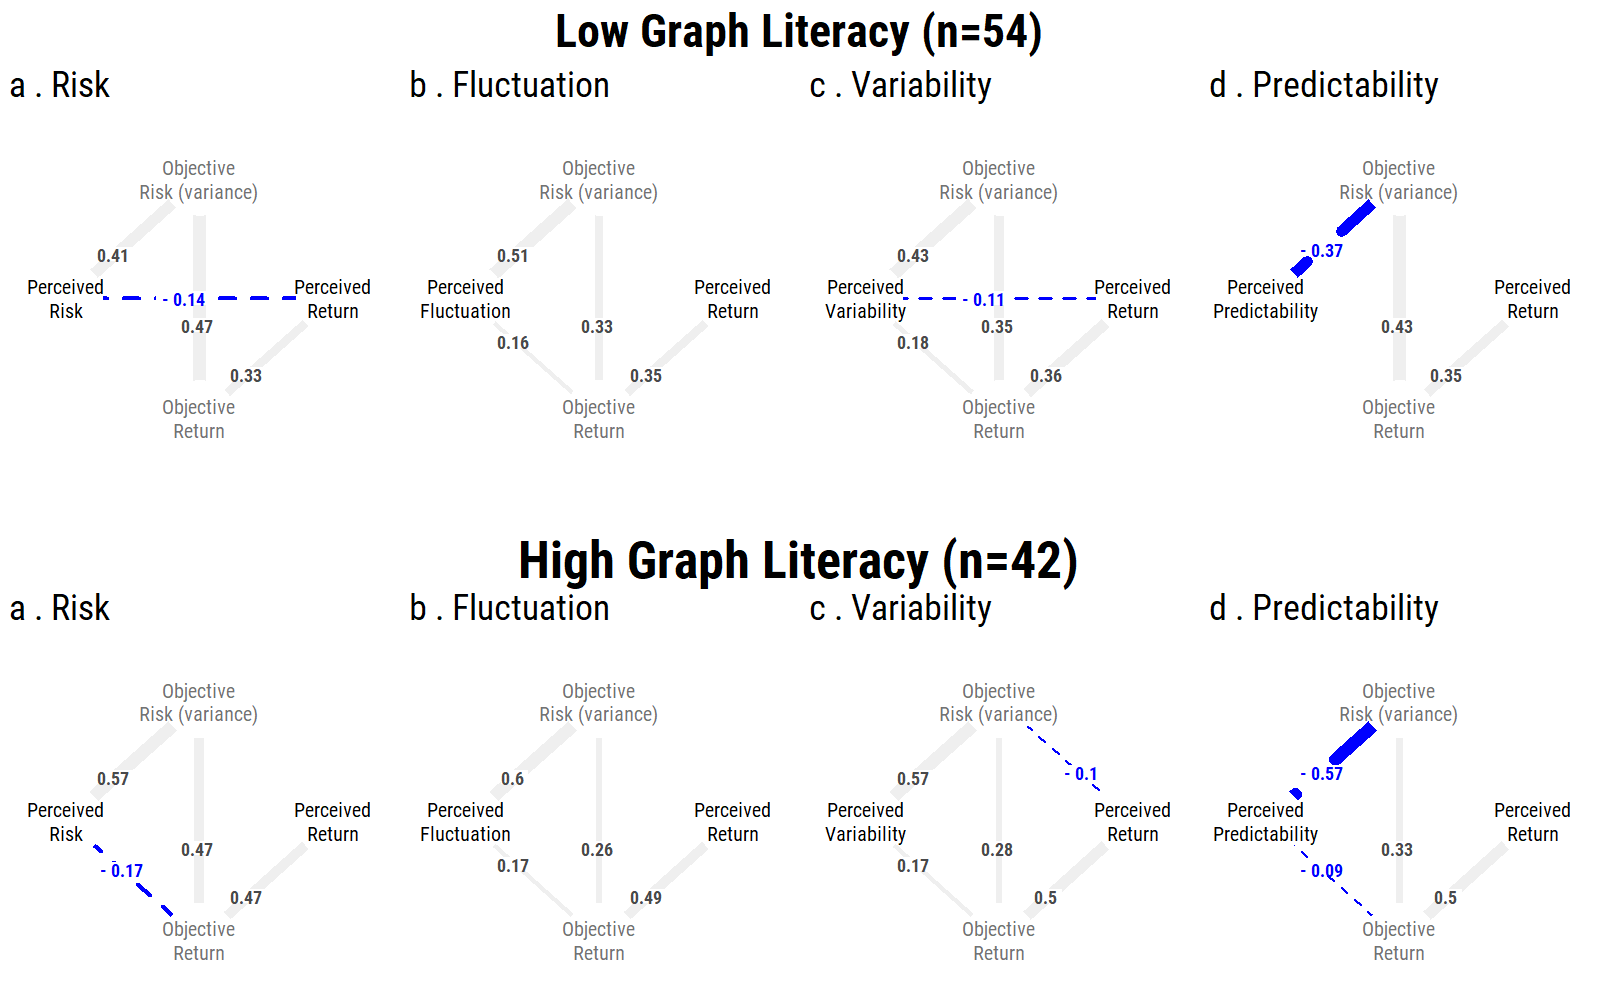
\includegraphics[width=.8\linewidth, keepaspectratio]{sfig1.png} 
 \caption{Partial correlation network. The methodology is similar to as described in the main text for Study 1, split by graph literacy. Only significant edges are shown, $\alpha=.01$.}
 \label{fig:study1_pcor_by_glit}
\end{figure}

\subsubsection{Robustness Check II: Stock market experience}
Figure~\ref{fig:study1_pcor_by_exp} shows the significant partial correlations after splitting the data into participants relatively inexperienced with the stock market and those with experience.
\begin{figure}[H] 
 \centering
 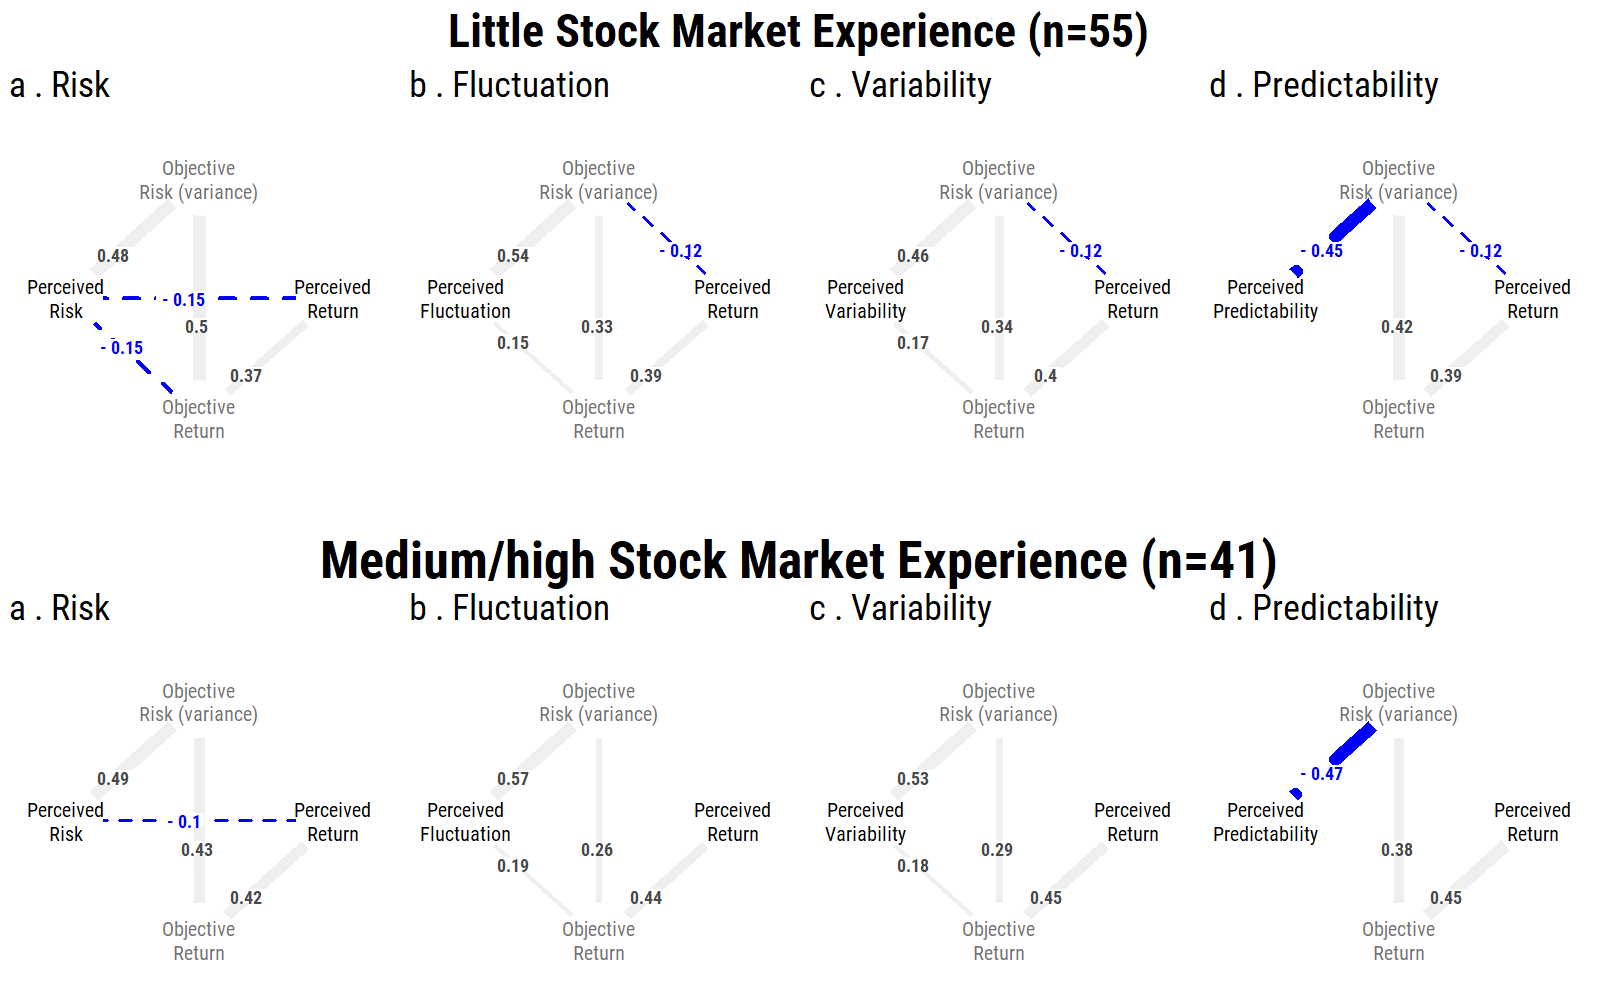
\includegraphics[width=.8\linewidth, keepaspectratio]{sfig2.png} 
 \caption{Partial correlation network. The methodology is similar to as described in the main text for Study 1, split by experience with the stock market. Only significant edges are shown, $\alpha=.01$.}
 \label{fig:study1_pcor_by_exp}
\end{figure}




%%%%%%%%%%%%%%%%%%%%%%%%%%%%%%%%%%%%%%%%%%%%%%%%%%%%%%%%%%%%%%%%%%%%%%%%%%%%%%%%%%%%%%%%%%





\section{Study 2 Supplementary Material}
\subsection{Materials Used in Study 2}
\label{tab:study2_material}
For Study 2, data from 1 January 2009 through 1 August 2017 from price indices of 23 stock markets corresponding to the world's most traded currencies (as of 2017) were obtained. Only price indices were used. Price indices calculate the value of the index based on the value of the stocks, excluding dividends. Table~\ref{tab:study2_material} lists the indices used in our study. Note: The HSI index (China-Hong Kong, Hang Seng Index) was excluded in favor of the Shanghai Stock Exchange Composite Index (SSE Composite), to avoid China being the only country to appear twice in the stimulus material. Also, the German DAX index was excluded in favor of the European EUROSTOXX index, which is also traded in euros. This table shows only the abbreviated version of the stimuli.
% latex table generated in R 3.5.0 by xtable 1.8-3 package
% Fri May 10 15:54:55 2019
\begin{table}[ht]
\centering\small
\caption{Stocks used in Study~2} 
\label{tab:study2_material}
\begin{tabularx}{.6\textwidth}{lcc}
  \toprule
Country & Index fund & ISIN \\ 
  \midrule
Europe & ES50 (EuroStoxx50) & EU0009658145 \\ 
  USA & DJIA & US2605661048 \\ 
  Japan & Nikkei225 & JP9010C00002 \\ 
  United Kingdom & FTSE100 & GB0001383545 \\ 
  Switzerland & SMI20 & CH0009980894 \\ 
  Australia & ASX & XC0009693018 \\ 
  Canada & TSX & XC0009695252 \\ 
  China-Shanghai & SSEC & CNM000000019 \\ 
  Sweden & OMXS30 & SE0000337842 \\ 
  Singapore & FSSTI & XC0009653640 \\ 
  India & BSE & XC0009698199 \\ 
  Russia & RTSI & RU000A0JPEB3 \\ 
  South Africa & JSE (JALSH) & --- \\ 
  Turkey & ISE100 & TRAIMKB00010 \\ 
  Poland & WIG20 & PL9999999987 \\ 
  Argentina & MERV & ARMERV160025 \\ 
  Indonesia & IDX & --- \\ 
  Malaysia & KLSE & --- \\ 
  Norway & OBX & NO0007035376 \\ 
  Mexico & MXX & --- \\ 
   \bottomrule
\end{tabularx}
\begin{tablenotes}
    \textit{Note.} ISIN $=$ International Securities Identification Number
\end{tablenotes}
\end{table}



\subsection{Supplementary Analyses, Study 2}
\label{sup:study2_results}
\subsubsection{Correlation coefficients}
\label{study2_subj_obj_cor}
Table~\ref{tab:study2_subj_obj_cor} shows the correlations between the objective variances of the returns of the index funds and the three perceptions of the variances: risk, fluctuation, and risk (measured as variance), pooled across participants and stimuli. This does not take the clustered nature of the data into account; see below for results controlling for the clustering. The simple correlation is highest for perceptions of fluctuation.
%
\begin{table}[H]
\begin{center}
\begin{threeparttable}
\caption{Study 2: Simple correlations between perceived risk and objective risk (variance)}
\label{tab:study2_subj_obj_cor}
\begin{tabular}{lrcrr}
\toprule
  & $r$ & 95\% CI & $t$ & $p$\\
 \midrule
& \multicolumn{4}{c}{Graph}\\
\cmidrule{2-5}
 Perceived risk (measured as variance) & $-.10$ & $[-.16$, $-.03]$ & $t(838) = -2.85$ & $.004$\\
 Perceived risk & $-.19$& $[-.26$, $-.12]$ & $t(798) = -5.54$& $<.001$\\
 Perceived fluctuation & $.19$ & $[.12$, $.25]$ & $t(798) = 5.41$& $<.001$\\
\midrule
 & \multicolumn{4}{c}{No graph}\\
 \cmidrule{2-5}
 Perceived risk (measured as variance) & $.19$ & $[-.26$, $-.12]$ & $t(778) = -5.47$& $ <.001$\\
 Perceived fluctuation & $-.39$ & $[-.44$, $-.33]$ & $t(798) = -11.81$& $ <.001$\\
 Perceived risk & $-.22$ & $[-.28$, $-.15]$ & $t(818) = -6.33$&  $ <.001$\\
\bottomrule
\addlinespace
\end{tabular}
\begin{tablenotes}[para]
\normalsize{\textit{Note.} CI = Confidence interval; Pearson correlations $r$ from pooled data; subjective values \textit{z} standardized at the individual level.}
\end{tablenotes}
\end{threeparttable}
\end{center}
\end{table}


\subsubsection{Study 2: Objective variance and subjective judgments, pairwise post hoc comparisons}
Table~\ref{tab:study2_hlm_trends_pairwise} shows the post hoc pairwise contrasts between the obtained regression coefficients, regressing objective variance on ratings of risk, fluctuation, and risk (variance), using Tukey \textit{p}-value adjustments. When graphs are shown, fluctuation perceptions are correlated strongest with the objective outcome variances of the index funds, compared with risk or risk (variance) perceptions, albeit the effect is small.
% latex table generated in R 3.6.0 by xtable 1.8-4 package
% Mon Jun 17 13:19:48 2019
\begin{table}[H]
\centering
\caption{Pairwise comparisons between trend coefficients with dependent variable: objective risk (variance of the index funds)} 
\label{tab:study2_hlm_trends_pairwise}
\begin{threeparttable}

    
    \begin{tabular}{lrrrrl}
      \toprule
    Contrast & $\Delta$ Slope & \textit{SE} & \textit{df} & $z$ Ratio & $p$ \\ 
      \midrule
      & \multicolumn{5}{c}{Graph}\\
      \cmidrule{2-6}
    Risk (variance)---fluctuation & -0.029 & 0.006 & Inf & -4.934 & $<$.0001 \\ 
      Risk (variance)---risk & 0.010 & 0.006 & Inf & 1.621 & .2366 \\ 
      Fluctuation---risk & 0.039 & 0.006 & Inf & 6.477 & $<$.0001 \\ 
       \midrule
       & \multicolumn{5}{c}{No graph}\\
       \cmidrule{2-6}
    Risk (variance)---fluctuation & -0.014 & 0.006 & Inf & -2.312 & .0542 \\ 
      Risk (variance)---risk & -0.006 & 0.006 & Inf & -0.991 & .5828 \\ 
      Fluctuation---risk & 0.008 & 0.006 & Inf & 1.344 & .3708 \\ 
       \bottomrule
    \end{tabular}
    \begin{tablenotes}
    \textit{Note.} Slope based on unstandardized effects; \textit{p}-value adjustment: Tukey for comparing three estimates. Inf $=$ Infinite.
    \end{tablenotes}
    \end{threeparttable}
\end{table}


% Table created by stargazer v.5.2.2 by Marek Hlavac, Harvard University. E-mail: hlavac at fas.harvard.edu
% Date and time: Mi., Mai 08, 2019 - 16:56:38
\begin{table}[!htbp] \centering \small
 \caption{Study 2: Linear mixed model results with dependent variable: objective variance of shown stocks} 
 \label{table:supplement_tab1} 
\begin{tabular}{@{\extracolsep{5pt}}lccc} 
\\[-1.8ex]\hline 
\hline \\[-1.8ex] 
 & \multicolumn{3}{c}{Unstandardized \textit{b} coefficients [range of dependent variable: 0.14--0.60]} \\ 
\cline{2-4} 
\\[-1.8ex] & (1) & (2) & (3)\\ 
\hline \\[-1.8ex] 
 Graph & $-$0.00 & $-$0.00 & \\ 
 & ($-$.01, .01) & ($-$.01, .01) & \\ 
 & $t$ = $-$0.00 & $t$ = $-$0.00 & \\ 
 & & & \\ \midrule
 Risk $\times$ No graph & .04 & & .05 \\ 
 & (.03, .05) & & (.04, .06) \\ 
 & $t$ = 9.59$^{***}$ & & $t$ = 16.89$^{***}$ \\ 
 & & & \\ 
 Risk (variance) $\times$ No graph & .03 & & .05 \\ 
 & (.03, .04) & & (.05, .06) \\ 
 & $t$ = 7.93$^{***}$ & & $t$ = 17.79$^{***}$ \\ 
 & & & \\ 
 Fluctuation $\times$ No graph & .05 & & .07 \\ 
 & (.04, .06) & & (.07, .08) \\ 
 & $t$ = 11.41$^{***}$ & & $t$ = 24.74$^{***}$ \\ 
 & & & \\ 
 Risk (all) $\times$ No graph & & .04 & \\ 
 & & (.04, .04) & \\ 
 & & $t$ = 16.62$^{***}$ & \\ 
 & & & \\ \midrule
 Risk$^{a}$ $\times$  Graph & .02 & .08 & \\ 
 & (.01, .03) & (.07, .08) & \\ 
 & $t$ = 3.69$^{***}$ & $t$ = 32.21$^{***}$ & \\ 
 & & & \\ 
 Risk (variance) $\times$ Graph & .02 & & \\ 
 & ($-$.001, .03) & & \\ 
 & $t$ = 1.89 & & \\ 
 & & & \\ 
 Fluctuation $\times$ Graph & .03 & & \\ 
 & (.01, .05) & & \\ 
 & $t$ = 3.74$^{***}$ & & \\ 
 & & & \\ \midrule
 Constant & .28 & .28 & .28 \\ 
 & (.28, .29) & (.28, .29) & (.28, .29) \\ 
 & $t$ = 121.40$^{***}$ & $t$ = 120.73$^{***}$ & $t$ = 170.06$^{***}$ \\ 
 & & & \\ 
\hline \\[-1.8ex] 
AIC weight$^{b}$ & 1.00 & 0.00 & 0.00 \\ 
AIC & -7,242 & -7,197 & -7,118 \\ 
BIC & -7,177 & -7,158 & -7,079 \\ 
LogLik & 3,631 & 3,604 & 3,565 \\ 
Random slope & no & no & no \\ 
Random intercept & participant & participant & participant \\ 
\hline 
\hline \\[-1.8ex] 
\multicolumn{4}{l}{\textit{Note.} $^{*}$ \textit{p} $<$ .05; $^{**}$\textit{p} $<$ .01; $^{***}$\textit{p} $<$ .001. Predictors are \textit{z} transformed.} \\
  \multicolumn{4}{l}{$^{a}$For Model 2, the predictor "risk" refers to all question wordings.} \\ 
 \multicolumn{4}{l}{$^{b}$Relative evidence strength, range 0 to 1 {\citep{Wagenmakers2004}}} \\
\end{tabular} 
\end{table} 



\subsubsection{Study 2: The risk--return paradox}
Table~\ref{tab:study2_rr} shows the simple correlation coefficients between the perceived return and the perceived risk/risk-as-variance/fluctuation. Note, correlations are pooled (ignoring the repeated-measure data structure) and simple (ignoring the intercorrelations between the risk and return variables in the data).
% latex table generated in R 3.6.0 by xtable 1.8-4 package
% Mon Jun 17 16:02:01 2019
\begin{table}[h!t]
\centering
\caption{Correlation between perceived risk and objective risk (variance)}
\label{tab:study2_rr}
\begin{tabular}{llrr}
 Graph & Question wording & $r$ [95\% CI] & Statistic \\ 
  \midrule
Graph & Risk (variance) & $-.10$, \  $[-.16$, $-.03]$ & $t(838) = -2.85$, $p = .004$ \\ 
   & Risk & $-.19$, \  $[-.26$, $-.12]$ & $t(798) = -5.54$, $p < .001$ \\ 
   & Fluctuation & $.19$, \  $[.12$, $.25]$ & $t(798) = 5.41$, $p < .001$ \\ 
   \midrule
No Graph & Risk (variance) & $-.19$, \  $[-.26$, $-.12]$ & $t(778) = -5.47$, $p < .001$ \\ 
   & Fluctuation & $-.39$, \  $[-.44$, $-.33]$ & $t(798) = -11.81$, $p < .001$ \\ 
   & Risk & $-.22$, \  $[-.28$, $-.15]$ & $t(818) = -6.33$, $p < .001$ \\ 
   \bottomrule
\multicolumn{4}{l}{{\textit{Note.} CI = Confidence interval. Pearson correlations $r$ from pooled data; subjective values \textit{z} standardized at the individual level.}}
\end{tabular}
\end{table}







\newpage
\subsection{Partial correlation coefficients}
Table~\ref{tab:study2_pcc} shows the numerical details of the partial correlation analysis, that is, the coefficients and the $p$ values from fitting the partial correlation networks (for implementation details, see main text). Shown are the coefficients for the perceived "risk," "fluctuation," and  "risk (measured as variance)" and returns of the index funds that were rated during Study~2.


\begin{sidewaystable}                                                                   

\begin{TableNotes}[para]                                                                                                                                        
\normalsize{\textit{Note.}  $^{*} = \textit{p} < .05; ^{**} = \textit{p} < .01; ^{***} = \textit{p} < .001$.}                                                                       
\end{TableNotes}                                                                                                                                                
                                                                                                                                                                
\small{                                                                                                                                                         
                                                                                                                                                                
\begin{longtable}{lllllllll}\noalign{\getlongtablewidth\global\LTcapwidth=\longtablewidth}                                                                      
\caption{Study 2 results: Partial correlations and \textit{p} values from the correlation networks                                                                      
\label{tab:study2_pcc}}\\                                                                                                                                           
\toprule                                                                                                                                                        
 \multicolumn{4}{c}{Graph} & \multicolumn{4}{c}{No graph}  &\\                                                                                        
\cmidrule(r){1-4} \cmidrule(r){5-8}                                                                                                                             
 & \multicolumn{1}{c}{1} & \multicolumn{1}{c}{2} & \multicolumn{1}{c}{3} & \multicolumn{1}{c}{4} & \multicolumn{1}{c}{1} & \multicolumn{1}{c}{2} & \multicolumn{1}{c}{3} & \multicolumn{1}{c}{4}\\                                                                                                                              
\midrule                                                                                                                                                        
\endfirsthead                                                                                                                                                   
\caption*{\normalfont{Table \ref{tab:} continued}}\\                                                                                                            
\toprule                                                                                                                                                        
 \multicolumn{4}{c}{With graph} & \multicolumn{4}{c}{Without graph}  &\\                                                                                        
\cmidrule(r){1-4} \cmidrule(r){5-8}                                                                                                                             
 & \multicolumn{1}{c}{1} & \multicolumn{1}{c}{2} & \multicolumn{1}{c}{3} & \multicolumn{1}{c}{4} & \multicolumn{1}{c}{1} & \multicolumn{1}{c}{2} & \multicolumn{1}{c}{3} & \multicolumn{1}{c}{4}\\                                                                                                                              
\midrule                                                                                                                                                        
\endhead                                                                                                                                                        
Risk &  &  &  &  &  &  &  & \\                                                                                                                                  
\ \ \ 1 Perceived risk &  &  &  &  &  &  &  & \\                                                                                                                
\ \ \ 2 Perceived return & $-.20^{**}$ &  &  &  & $-.14$ &  &  & \\                                                                                           
\ \ \ 3 Objective risk (variance) & $\hphantom{-}.44^{***}$ & $-.01$ &  &  & $\hphantom{-}.13^{***}$ & $\hphantom{-}.02$ &  & \\                            
\ \ \ 4 Objective return & $-.13^{**}$ & $\hphantom{-}.32^{***}$ & $\hphantom{-}.55^{***}$ &  & $\hphantom{-}.02$ & $-.02$ & $\hphantom{-}.58^{***}$ & \\ 
\ \ \ 5 Positive attitude & $-.09^{*}$ & $\hphantom{-}.16^{***}$ & $\hphantom{-}.03$ & $-.21^{***}$ & $-.17^{***}$ & $\hphantom{-}.27^{***}$ & $-.01$ & $-.11^{**}$\\                                                                                                                                                   
Risk-as-variance &  &  &  &  &  &  &  & \\                                                                                                                      
\ \ \ 1 Perceived risk-as-variance &  &  &  &  &  &  &  & \\                                                                                                    
\ \ \ 2 Perceived return & $-.19^{**}$ &  &  &  & $-.11$ &  &  & \\                                                                                           
\ \ \ 3 Objective risk (variance) & $\hphantom{-}.51^{***}$ & $\hphantom{-}.05$ &  &  & $\hphantom{-}.13^{**}$ & $\hphantom{-}.00$ &  & \\                  
\ \ \ 4 Objective return & $-.10^{*}$ & $\hphantom{-}.38^{***}$ & $\hphantom{-}.53^{***}$ &  & $\hphantom{-}.08^{*}$ & $-.05$ & $\hphantom{-}.57^{***}$ & 
\\                                                                                                                                                              
\ \ \ 5 Positive attitude & $-.13^{**}$ & $\hphantom{-}.13^{**}$ & $-.03$ & $-.13^{***}$ & $-.11^{*}$ & $\hphantom{-}.29^{***}$ & $-.01$ & $-.08^{*}$\\ 
Fluctuation &  &  &  &  &  &  &  & \\                                                                                                                           
\ \ \ 1 Perceived fluctuation &  &  &  &  &  &  &  & \\                                                                                                         
\ \ \ 2 Perceived return & $\hphantom{-}.07$ &  &  &  & $-.22^{***}$ &  &  & \\                                                                               
\ \ \ 3 Objective risk (variance) & $\hphantom{-}.65^{***}$ & $-.10^{*}$ &  &  & $\hphantom{-}.17^{***}$ & $-.02$ &  & \\                                   
\ \ \ 4 Objective return & $\hphantom{-}.04$ & $\hphantom{-}.37^{***}$ & $\hphantom{-}.38^{***}$ &  & $\hphantom{-}.05$ & $-.08$ & $\hphantom{-}.56^{***}$ & \\                                                                                                                                                           
\ \ \ 5 Positive attitude & $-.09^{*}$ & $\hphantom{-}.06$ & $\hphantom{-}.05$ & $-.15^{***}$ & $-.15^{**}$ & $\hphantom{-}.29^{***}$ & $-.03$ & $-.09^{*}$\\                                                                                                                                                           
\bottomrule                                                                                                                                                     
\addlinespace                                                                                                                                                   
\insertTableNotes                                                                                                                                               
\end{longtable}                                                                                                                                                 
                                                                                                                                                                
}

\end{sidewaystable}






\subsubsection{Linear model comparison for perceived return}
Data-driven selection of the (hierarchical) linear model that we used in the main text was based on complexity-penalized goodness of fit (Akaike information criterion). Dependent variable was perceived return, and the fixed effects were Question $\times$ Perceived Variance, Graph $\times$ Perceived Variance, objective variance, and objective return. Predictors question and graph were effects coded. The random effects structure is varied: See the different rows in Table B7, where Row 1 contains a fixed-effects-only model and the last row the maximum random effects structure of interest. For all models, variance inflation factors ($VIF$) were at maximum 2 ($VIF > 5$ indicates problematic multicollinearity). Table \ref{sup:tab:study2_attitude_lm_trends} further displays the mixed-effects modeling results including the predictor attitudes.
% latex table generated in R 3.6.0 by xtable 1.8-4 package
% Fri Jun 21 08:49:47 2019
\begin{table}[H]
\centering
\caption{Study 2: Linear model comparison with dependent variable: perceived return} 
\label{tab:study2_lm_return_modelcomparison}
\begin{tabular}{p{4.3cm}cccccccr}
  \toprule
 & \textit{df} & AIC & BIC & LogLik & Deviance & $\chi^2$ & $\chi^2$\textit{df} & Pr(>$\chi^2$) \\ 
  \midrule
Fixed effects only & 10 & 14,791 & 14,855 & -7,385 & 14,771 &  &  &  \\ 
  Interc. by id & 11 & 14,504 & 14,575 & -7,241 & 14,482 & 289 & 1 & 0.000 \\ 
  Interc. by index & 11 & 14,612 & 14,683 & -7,295 & 14,590 & 0 & 0 & 1.000 \\ 
  Interc. \& slope by id & 13 & 13,517 & 13,601 & -6,745 & 13,491 & 1,099 & 2 & 0.000 \\ 
  Interc. \& slope by index & 13 & 14,611 & 14,695 & -7,293 & 14,585 & 0 & 0 & 1.000 \\ 
  Interc. \& slope by id + interc. \& slope by index & 16 & 13,308 & 13,412 & -6,638 & 13,276 & 1,309 & 3 & 0.000 \\ 
   \bottomrule
   \multicolumn{9}{l}{\small\textit{Note}. Variables were centered at the Likert scale midpoints. AIC = Akaike information criterion; BIC = Bayesian information criterion, id = participant identifyer, interc = intercept.}\end{tabular}
\end{table}


\begin{table}[H]
\begin{center}
\begin{threeparttable}
\caption{Study 2 results: Mixed-effects model with estimated slopes for the predictor attitude. Dependent variable: perceived return}
\label{sup:tab:study2_attitude_lm_trends}
\begin{tabular}{lccrrr}
\toprule
Question & Slope & \textit{SE} & \textit{df} & \textit{z} Ratio & \textit{p}\\
\midrule
& \multicolumn{5}{c}{No Graph}\\
\cmidrule{2-6}
Risk & 0.344 & 0.044 & \$\textbackslash{}infty\$ & 7.819 & .000\\
Risk (measured as variance) & 0.358 & 0.043 & \$\textbackslash{}infty\$ & 8.323 & .000\\
Fluctuation & 0.448 & 0.047 & \$\textbackslash{}infty\$ & 9.511 & .000\\
\midrule
& \multicolumn{5}{c}{Graph}\\
\cmidrule{2-6}
Risk & 0.145 & 0.041 & \$\textbackslash{}infty\$ & 3.501 & .000\\
Risk (measured as variance) & 0.085 & 0.041 & \$\textbackslash{}infty\$ & 2.087 & .037\\
Fluctuation & 0.077 & 0.038 & \$\textbackslash{}infty\$ & 2.058 & .040\\
\bottomrule
\end{tabular}
\begin{tablenotes} \small
    \textit{Note.} Model specification as in Footnote 12 of the main text, but adding to the fixed effects the attitude score as main effect and as interaction term.
\end{tablenotes}
\end{threeparttable}
\end{center}
\end{table}


\end{document}
 